
\documentclass[a4paper,12pt]{report}
\usepackage[french]{babel}
\usepackage{graphicx}
\usepackage{lipsum}% just to generate text for the example
\usepackage[hidelinks]{hyperref} % san li, ou pap ka al directement sou yon chap
% a partir de table des matieres lan or al sou yon link internet automatiquement


\usepackage{lmodern}
\usepackage{titlesec}
\usepackage{microtype}
\usepackage{tikz}


\definecolor{myblue}{RGB}{0,82,155}

\titleformat{\chapter}[display]
  {\normalfont\bfseries\color{myblue}}
  {\filleft%
    \begin{tikzpicture}
    \node[
      outer sep=0pt,
      text width=2.5cm,
      minimum height=3cm,
      fill=myblue,
      font=\color{white}\fontsize{80}{90}\selectfont,
      align=center
      ] (num) {\thechapter};
    \node[
      rotate=90,
      anchor=south,
      font=\color{black}\Large\normalfont
      ] at ([xshift=-5pt]num.west) {\textls[180]{\textsc{\chaptertitlename}}};  
    \end{tikzpicture}%
  }
  {10pt}
  {\titlerule[2.5pt]\vskip3pt\titlerule\vskip4pt\LARGE\sffamily}

\begin{document}

\begin{figure}[t]
        \centering
        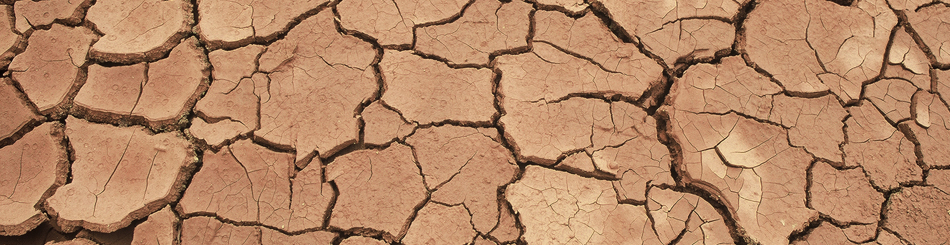
\includegraphics[width=2\textwidth]{image_fond}
        \label{image-GIS}
        \end{figure}

\title{GéoTech}
\author{
        DUBUCHE Kevin J. \\
        Faculté Des Science de l'Université d'Etat Haïti\\
        270, Angle Rues Mgr. Guilloux et Joseph Janvier\\
        Port-au-Prince, B.P: 1385 \underline{Haïti}
        \and
        THEODORE Barbara G.\\
        Faculté Des Science de l'Université d'Etat Haïti\\
        270, Angle Rues Mgr. Guilloux et Joseph Janvier \\
        Port-au-Prince, B.P: 1385  \underline{Haïti}
}
\date{\today}
\maketitle

\pagenumbering{roman}
\tableofcontents
\newpage
\pagenumbering{arabic}

\section{Résumé}
\paragraph{}
L'objectif principal de ce projet est de créer une base de données géotechniques
 accessible par Internet. Cette base de données permettra de mutualiser les données 
 sur le sous-sol accumulées par différents organismes, tant publiques que privées, 
 au cours de ces 50 dernières années. Cette application Web constitue donc un espace 
 partagé permettant à ces différents organismes de centraliser et de gérer une banque 
 de données géotechniques.


\paragraph{Abstract}
The main objective of this project is to create a geotechnical database
 accessible via the Internet. This database will make it possible to pool data
 on the basement accumulated by various organizations, both public and private,
 over the past 50 years. This web application therefore constitutes a space
 shared allowing these different organizations to centralize and manage a
 geotechnical database.
\\
\\
\\
\\
\\
\\
\par
 {\small 
 La totalité des codes est disponible en ligne sur GitHub : \url{https://github.com/geotech}.
L’application est accessible via l’adresse: \url{https://geotech.ht}

 }

\chapter*{Remerciements}
\addcontentsline{toc}{chapter}{Remerciements}
\paragraph{}
Ce projet de fin d’études représente l'aboutissement de notre formation d’ingénieur électronique. 
Nous tenons à réserver ces quelques lignes pour exprimer notre
reconnaissance aux personnes qui nous ont apporté leur support pour réaliser ce travail :

\begin{itemize}
    \item Merci à l'URGéo pour nous avoir fait confiance et donné ce formidable projet;\par
    \item Merci à nos encadreurs en chef: M Dominnique Boisson et Mme Tayana Étienne pour \par
    \item Merci à nos tuteurs directs M Kelly Guerrier et M Karl Henry Victor pour leurs 
    jugements très fructueux et leur encadrement général;\par
    \item Merci à  M Elysée Villiard pour l'encadrement (programmation et base de données);\par
    \item Merci à Mme Anne Doris Vital pour l'encadrement (sécurité informatique);\par
    \item Merci à l'URGéo et la MBDS pour l'encadrement général;\par
    \item Merci aux professeurs Jacques Faubert Etienne, ...;\par
    \item Merci au stagiaire Droogleever Fortuyn Mélanie Sarah pour ses commentaires 
    très précieux à chaque étape et son implication sans précédent; \par
    \item Merci à nos beta testeurs ...;\par
    \item Merci aux partenaires: KAYTEK, MBDS, ...;\par
    \item Merci à la communauté FDS pour tout ce qu'elle nous a appris tant 
    moralement que professionnellement;\par
    \item Merci à Rodmy G. Sully Guerrier, ... pour leur aide précieuse au niveau du document; \par
\end{itemize}


\section{Glossaire}
\paragraph{URGéo :}
L'Unité de Recherche en Géosciences a pour mission de mener des
recherches dans les domaines des géosciences où elle a les capacités
pour le faire.Cela implique une bonne compréhension des différentes 
problématiques liés au sol et au sous-sol et la proposition de moyens
de mitigations adaptées à la réalité haïtienne.
\\
Pour le moment, l’URGéo constitue l’une des rares unités de recherches
dédiée aux géosciences dans le pays. Ces chercheurs prennent part à de
grandes réunions savantes et scientifiques en Amérique du Nord, en 
Europe et dans les Caraïbes.

\paragraph{BME}
Le Bureau des Mines et de l’Energie est un organisme autonome créé en 
1986 fonctionnant sous la tutelle du Ministre des Travaux Publics, Transports 
et Communications (MTPTC). Sa mission principale est de promouvoir la recherche
et l'exploitation des ressources minérales et énergétiques d'Haíti ainsi que les 
techniques appropriées y relative.

\paragraph{SICOD}
La  Société d’Ingénierie Constructions et d’Orientations Diverses,
fondée en 2011, est une société haïtienne en noms collectifs qui évolue dans 
les domaines d’ingénierie géotechnique et de constructions.
Il s'adonnent aux prélèvements des données des essais de laboratoire, des 
interprétations systématiques et aux recommandations techniques. 
Ils apportent leur support technique aux maîtres d'ouvrages dans la réalisation 
de leur chantier tout en observant les critères techniques de l'art.

\paragraph{LNBTP}
Le Laboratoire National Du Bâtiment et des Travaux Publics est une institution publique à gestion autonome chargée du contrôle de
la qualité des infrastructures en construction dans le pays. Il s'occupe 
aussi des études géotechniques, des recherches appliquées sur les matériaux de 
construction et de la promotion des normes en matière de génie civil.

\paragraph{Géothechsol}
Géothechsol est un Bureau d’Etudes 
en Ingénierie Géotechni\-que et Environnemental
ainsi qu’en formulation de béton et ses essais mécani\-ques et physiques, qui s’est
fixé pour objectif de vous apporter une réponse sérieuse et de qualité, adaptée à 
vos besoins dans le respect de vos contraintes. Ce bureau axe ses travaux sur les
essais géotechniques et des sondages.

\paragraph{SIG ou GIS :}  
Un système d'information géographique ou SIG (en anglais, Geographic 
Information System) est un système d'information conçu pour 
recueillir, stocker, traiter, analyser, gérer et présenter tous les 
types de données spatiales et géographiques. 



\paragraph{BRGM :}
Bureau de Recherches Géologiques et Minières


\paragraph{PDF :}
Portable Document Format. Le format PDF permet de conserver en 
toutes circonstances la mise en page 
originelle d'un document, quel que soit le logiciel ou le système 
d'exploitation utilisé pour l'ouvrir. Créé par la société Adobe, 
il est aujourd'hui très utilisé à travers le monde.

\paragraph{ISO :}
International Organization for Standardization.
L'Organisation internationale de normalisation généralement désigné sous son
 sigle : ISO, est un organisme de normalisation international composé de 
 représentants d'organisations nationales de normalisation de 164 pays.


\paragraph{CSV :}
Un fichier CSV (en anglais, Comma Separated Values) est le fichier de 
base des données recueillies - sans formatage particulier. Chaque 
champ est séparé par une virgule.

\paragraph{UI :}
L’UI design est directement lié à l’UX design. Cela signifie interface 
utilisateur. Il s’agit du lien direct entre l’utilisateur (donc le visiteur) 
et la machine (le programme ou la plateforme qui a permis de construire 
votre site web). De nombreux éléments entrent dans l’UI design et vous 
les connaissez certainement : la typographie, la police, la taille et la 
couleur d’écriture, les visuels, la charte graphique, identité visuelle, 
charte éditoriale, ou l’intuitivité.

\paragraph{UX :}
UX Design ou expérience utilisateur est un ensemble de techniques 
permettant de concevoir un site internet dans lequel le visiteur navigue 
de manière optimale. Le but est d’améliorer l’interaction entre l’homme 
et la machine. 

\paragraph{WGS84 :}
World Geodesic System (Sytème géodésique mondial) - révision de 1984
C'est un système de coordonnées terrestres, basé sur un géoïde de référence 
prenant la forme d'un ellipsoïde de révolution.
WGS84 est un système de coordonnées comprenant un modèle de la terre. Il est 
défini par un ensemble de paramètres primaires et secondaires :
les paramètres primaires définissent la forme de l'ellipsoïde de la terre, sa vitesse angulaire, et sa masse.
les paramètres secondaires définissent un modèle détaillé de la pesanteur terrestre.



\chapter{Contexte}

\chapter*{Introduction}
Depuis la naissance de l'informatique géologique (an-
nie 1970), toutes les études qui ont été faites dans ce
domaine ont été orientées vers la recherche des
méthodes les plus fiables et les moins coûteuses pour
stocker, traiter et restituer les données géologiques et
géotechniques concernant les 3 sujets suivants :
\paragraph{programmes de base de données (ou banque de
données) }: dont l'objectif est le stockage des donn6es;

\paragraph{programmes de calculs}
 dont l'objectif est le traite-
ment mathématique, statistique et éventuellement géo-
statistique des données;

\paragraph{programrnes de cartographie}
 dont l'objectif est la
restitution des données géologiques et géotechniques
sous forme graphique.
\par
Historiquement, le stockage des données géologiques
et géotechniques a été fait sur des fichiers séquentiels
spécialisés dont chacun ne présente qu'une application.
\par
La redondance des données (répétition des mêmes
données dans des fichiers différents) était é1evée, et il
n'y avait pas une indépendance entre les données et les
programmes de traitement. I1 était aussi nécessaire de
codifier de faqon externe et interne les données géologiques pour les stocker. C'est seulement en utilisant
des systèmes de gestion de base de données généraux
qu'on a pu diminuer la redondance entre les données
et assurer l'indépendance des programmes.
\par
 Au début,
les auteurs ont considéré que les données de notre
domaine pouvaient avoir une structure hiérarchique
(base de données arborescente). A la suite de l'échec
de ce type de base de données, on a travaillé sur des
bases de données en réseau. Ces deux types de base de
données n'ont pas pu éliminer d'une faqon définitive
la redondance et surtout la codification interne des
données géologiques.
\cite{tunis}
\par
Pour atteindre cet objectif, assurer une indépendance
totale entre les données et les programmes de traitement et obtenir une base de données géologiques et
géotechniques très souple, nous utilisons, pour la
conception de << GEO-TECH>>, le système
de gestion de base de données relationnel général en
considérant que toutes les données pouvaient être
modé1isées sous forme de tableaux  dont
l'une des colonnes est la clef. Chaque colonne sera un
domaine géologique ou géotechnique et chaque ligne (tuple)
un enregistrement.

\chapter{Contexte}
    \section{Introduction}
        
    \paragraph{}
    Ce mémoire s'incrit dans le cadre d'une collaboration entre
    l'URGéo et Kay Nou Tek. Ce projet est financé par l’Ambassade
    de Suisse en Haïti et a pour objectif d’explorer le potentiel 
    du numérique pour améliorer les pratiques de construction.
    Le but principal de ce travail est
    d'apporter une solution téchnologique  qui facilitera la 
    gestion des données géotechniques en Haïti.
    \paragraph{}
    Ce document comporte deux grandes parties: une première axée
    sur la théorie, se focalisant sur le contexte et les avantages
    de la réalisation d'un tel projet. La seconde partie est plus pratique
    et combine le travail de l'ingénieur logiciel et des analystes programmeurs responsables
    du projet.
    \begin{figure}
        \centering
        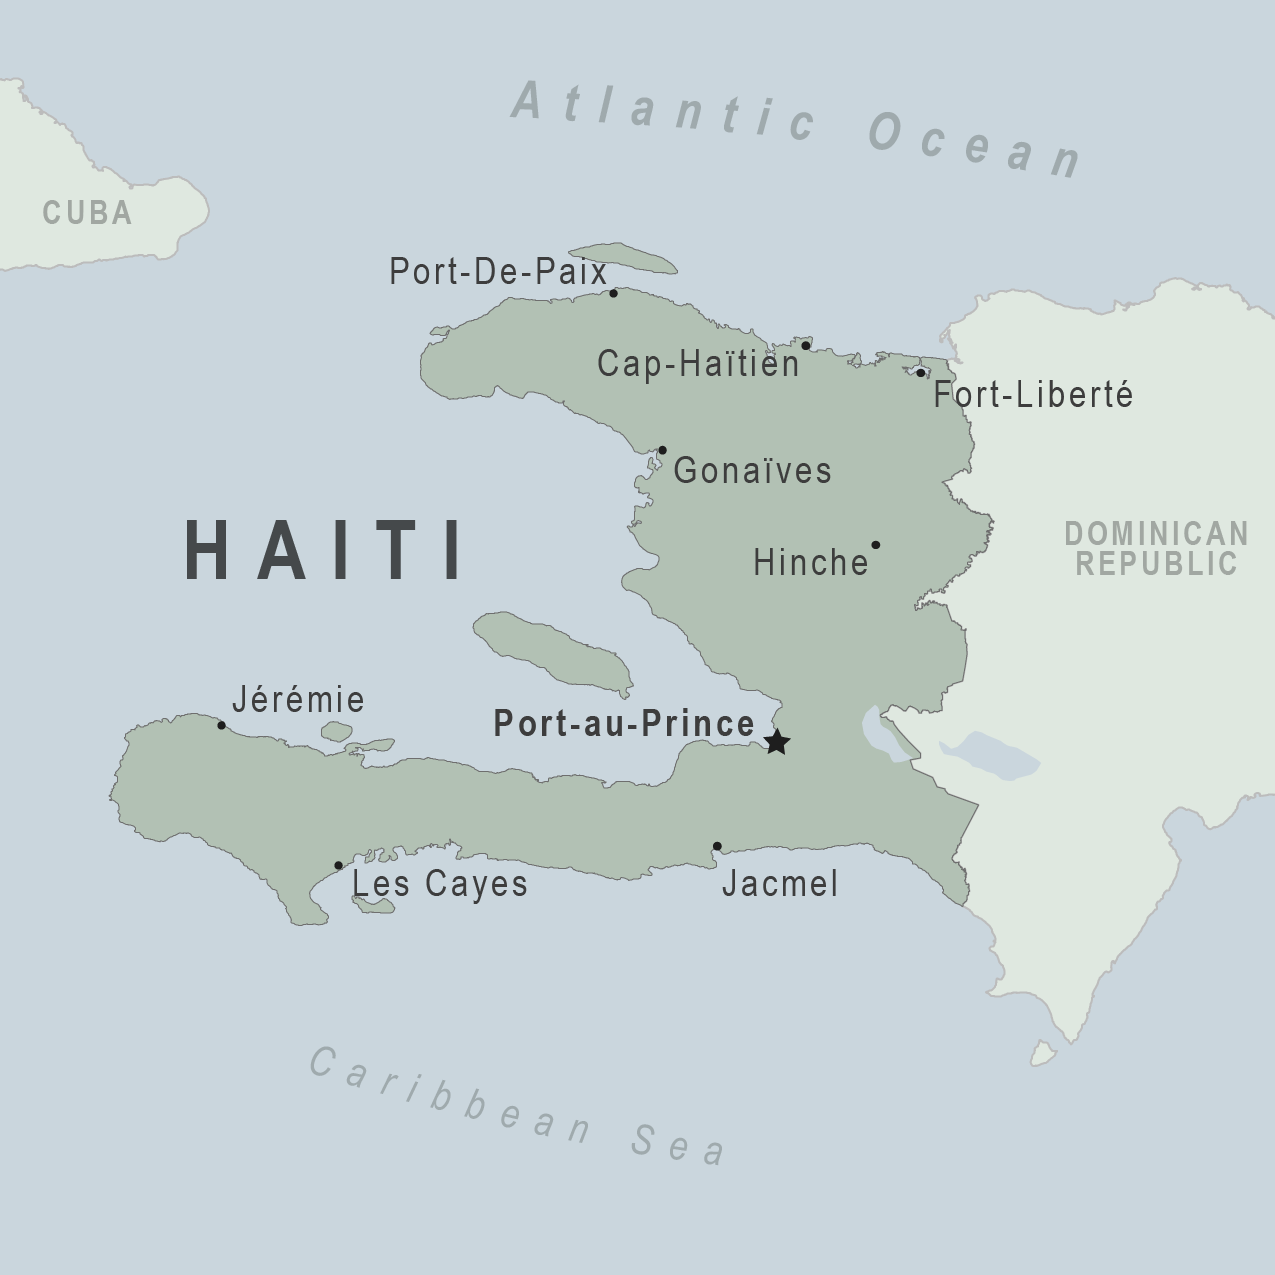
\includegraphics[width=1\textwidth]{images/Contexte/map-haiti.png}
        \caption{Cartographie d'Haïti}
    \end{figure}
        \subsection{Généralités}
            \subsubsection{La géotechnique, pourquoi est-ce important ?}
            \par 
La \textbf{géotechnique} est l’ensemble des 
activités liées aux applications de la mécanique des sols, de la mécanique 
des roches et de la géologie de l’ingénieur\footnote{
    Définition selon l’Union syndicale géotechnique accessible via ce lien: 
    \url{http://u-s-g.org/profession-geotechnicien.asp?idpage=1}}.
Au cours d'un projet d'aménagement, dans le but d'assurer  la fiabilité et la durabilité
des ouvrages, le constructeur est dans l'obligation de prendre en compte
la nature du sous-sol du site où il est prévu de construire.

Il s'agit en fait d'adapter le projet au site envisagé.
\par
La mission du géotechnicien consiste principalement à \cite{Chamel}\cite{benachenhou2019approche}:
\begin{itemize}
    \item définir les cadres géologique, hydrogéologique et topographique 
    du site étudié ;
    \item définir les aléas existants vis-à-vis des risques naturels : 
    détection des cavités, stabilité général d’un site (par rapport au 
    glissement de terrain par exemple), sismicité.
    \item définir les terrassements : faisabilité, réemploi des matériaux, 
    tenus des talus et parois des fouilles ;
    \item définir l’influence des circulations d’eaux souterraines, 
    agressivité de l’eau vis-à-vis des bétons ;
    \item définir comment la nature et la répartition des 
    formations géologiques pourrait influencer la réalisation des travaux et la conception 
    de l’ouvrage.
\end{itemize}
\paragraph{}
En général, le géotechnicien résume sa mission dans un rapport.
Ce rapport comprend les résultats des différents tests (Figure \ref{fig:test_penetrometrique}) 
réalisés : essais de pénétration, forages, essais de laboratoire,
essais géophysiques, etc.
\begin{figure}
    \centering
    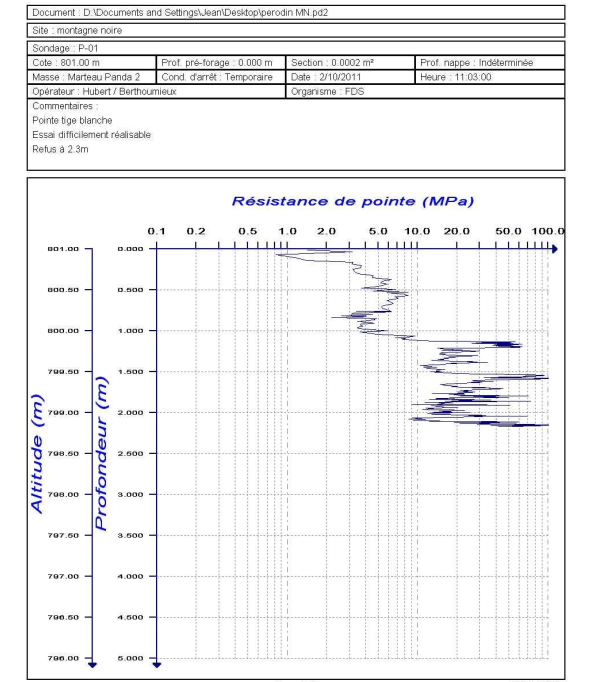
\includegraphics[width=0.5\textwidth]{images/Contexte/penetrographe.png}
    \caption{Exemple de résultat d'un essai pénétrométrique dynamique }\cite{penetrometrie}
    \label{fig:test_penetrometrique}
\end{figure} 

Ce rapport est rédigé non seulement dans le but d’informer le client sur la nature des interventions
, mais aussi d’exposer les principaux résultats des tests recueillis, de façon à mener à bien
l’exécution des projets.
\par
La zone d'étude de ce projet correspond à Haïti (Figure \ref{fig:haiti}).
\begin{figure}
    \centering
    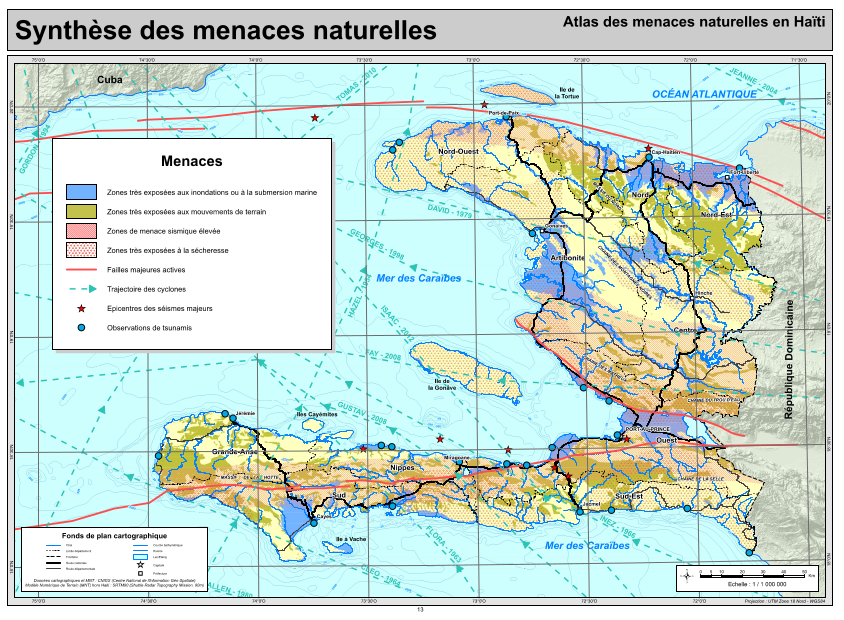
\includegraphics[width=1\textwidth]{images/Contexte/haiti.png}
    \caption{Cartographie d'Haïti, Synthèse des menaces naturelles  \cite{ciat}}
    \label{fig:haiti}
\end{figure}
Ce pays situé dans les Caraïbes a une superficie de  \SI{27750}{\kilo\metre\squared}\cite{superficie}.
L'importance des données géotechniques s'est montrée incontournable dans ce pays particulièrement 
après un séisme dévastateur en Janvier 2010.

\paragraph{}
Vulgairement appelé \textit{Goudougoudou}, un séisme de magnitude 7\cite{mondiale2010haiti} sur l'échelle de Richter, 
a fait de grands ravages sur l'île. Les pertes enregistrées, tant en vies humaines qu'en biens
matériels, ne faisaient que refléter l'ignorance de certains et le laisser-aller des autres. 
Des bâtiments construits défavorablement, des ravines devenues des villages ou simplement des 
constructions effectuées sur un sol inadéquat; telles étaient les causes majeures de ces 
pertes. En Haïti, le plus souvent les constructions sont pris à la légère.
\textit{
    Un recensement national en 2003 a rapporté que 8\% des bâtiments dans les zones urbaines d'Haïti sont
    les bidonvilles (Figure : \ref{fig:bidonville})    
    , connus sous le nom de kay atè, et 78\% des maisons sont 
    des maisons en blocs 
    de béton à un étage ou à plusieurs étages \cite{desroches2011overview}.} 
    \begin{figure}
        \centering
        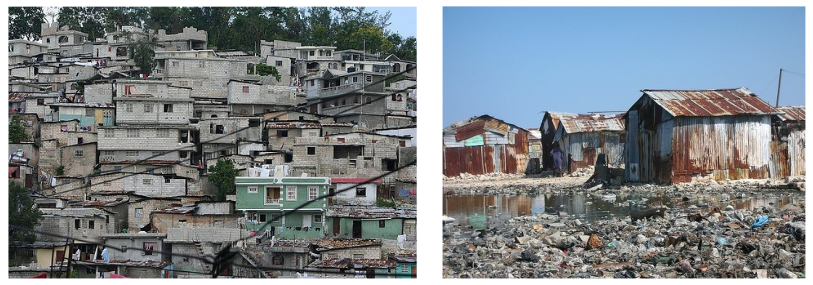
\includegraphics[width=1\textwidth]{images/Contexte/bidonville.png}
        \caption{Bidonvilles aux alentours de Port-au-Prince  \cite{holly1999problemes}}
        \label{fig:bidonville}
    \end{figure}
L' image \ref{fig:musseau} est une représentation typique
 des nombreux exemples de dégâts causés par un glissement de terrain à Musseau en 2008.
 \begin{figure}
    \centering
    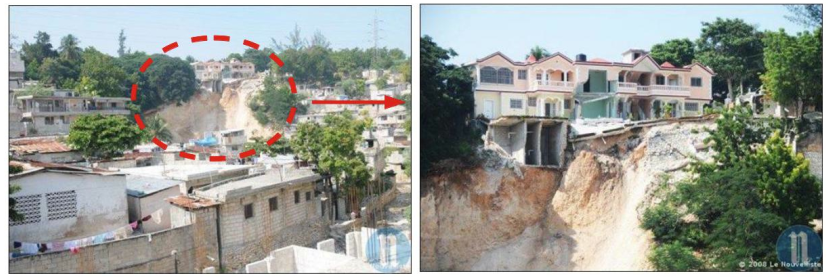
\includegraphics[width=1\textwidth]{images/Contexte/musseau.png}
    \caption{Glissement de terrain à Musseau (photo Le Nouvelliste)}
    \label{fig:musseau}
\end{figure}
\paragraph{}
Le tremblement de terre du 12 Janvier 2010 a ravagé le pays en
tuant plus de 200000 personnes, détruisant
105 000 bâtiments et endommagé 280 000 bâtiments \cite{mondiale2010haiti}.
Ce qui a abouti à près d'un million de sans-abris selon  le journal 
\textit{Natural Hazards and Earth System Sciences Discussions} \cite{daniell2013uncovering}.
Avec une 
étude de sol et des données géotechniques adéquates, un ingénieur pourrait orienter son travail
en connaissance de cause. Par conséquent, depuis maintenant une bonne décennie, les demandes
se multiplient pour l'accès à ces informations.  




            \subsubsection{Production et gestion des données géotechiques en Haïti}
                \par
Les outils papiers utilisés pour le moment sont très vulnérables à des
catastrophes comme des incendies ou des tremblements de terre. La perte 
des documents de référence entraînerait un travail
colossal pour le recouvrement des informations relatives à chaque 
dossier.
\par
Diverses instances détiennent les données recueillies au cours
de leurs études géotechiques respectives. 
Ainsi, lorsqu’un particulier a besoin de faire des études de sols, il 
fait appel à des instances clés capables de les prendre en charge. 
Parmi elles que nous avons pu contacter ou avec lesquels nous avons fait un partenariat, citons :
\begin{itemize}
    \item \textbf{URGéo}
    Unité de Recherche en Géosciences 
    \item \textbf{BME}
    Bureau des Mines et de l’Energie
    \item \textbf{SICOD}
    Société d’Ingénierie Constructions et d’Orientations Diverses
    \item \textbf{LNBTP}
    Laboratoire National Du Bâtiment et des Travaux Publics 
    \item \textbf{Géothechsol}
    \item \textbf{Insolflor}
\end{itemize}   

\par
En général ces entreprises s'impliquent dans la construction et la recherche. 
Leur travail consiste à effectuer une reconnaissance/étude géotechnique des sites .
Depuis plusieurs années ils se sont faits remarqués, notamment dans
l'étude des sols avant la construction de grands bâtiments. Ils sont aussi impliqués
dans la réalisation de ponts et de routes sur le territoire
haitien. 
\paragraph{}
Cepandant un problème persiste: les données recueillies par ces instances
ne sont nullememt en sécurité car elle sont stockées sur papier.
De plus, le minimum qui est numérisé n'est pas intégré dans un environnement 
dédié à cela.
L'analyse des données géotechiques sur toute l'étendue du territoire devient
encore plus difficile car aucune instance ne dispose de l'integralité des tests effectués.
Cela implique une exploitation non optimale de ces données.
\paragraph{Les problèmes actuelles}
\paragraph{}
Le plus grand inconvénient dans la gestion actulles des données géotechiques
en Haïti est la sécurité de ces dernières. 
Cet aspect n'est pas anodin et doit être pris en compte dans la gestion d'un système
d'information.
Actuellement, les critères fondamentaux de la securité des données ne sont nullememt en vigueur en dans le cadre des 
des Systèmes d'Information Géotechniques.
\paragraph{Confidentialité : }
On n'a aucune garantie que seules les personnes autorisées 
aient accès aux données géotechiques. Le fait qu'elles soient
stockées que sur papier auguemente les risques qu'une personnes
n'ayant pas le droit d'accès puisse s'acquérir de ces données.
\paragraph{Intégrité : }
Actuellement personne ne peut
garantir que les données géotechniques que l'on a en notre possession 
sont bien celles que l’on croit. L'intégrité n'est pas assurée car le risque
pour que les données géotechniques soit altérées est trop grand.
\paragraph{Disponibilité :}
C'est l'un des plus grand inconvénient de la gestion actuelle des 
données géotechniques. Trouver une étude qui a été réalisée dans un endroit précis
ou à une date pricise n'est pas évidente. Cela coûte beaucoup de temps et de ressource pour effectuer
les recherche. Par conséquent, le facteur de disponibilité n'est pas 
au rendez-vous car le délai d'acces aux informations est trop long.

\paragraph{}
Divers autres problèmes peuvent être constatés dans la gestion
des données géotechniques en Haïti. Notemment le fait que ces données
ne soient pas à l'abrit des catastrophes humaines (sabotage) et naturelles
(incendies, tremblement de terre, inondation, etc).


\par    
\begin{table}
        \centering
        \begin{tabular}{|p{0.10\linewidth}|p{0.80\linewidth}|}
        \hline
                \textbf{No} & \textbf{Problèmes} \\
                \hline
                    1&
                    Non disponibilité des données
                         \\
                \hline
                2&
                Données susceptibles aux catastrophes humaines et naturelles.
                    \\
                \hline
                3&
                Risques de récidive des réalisations de test
                    \\
                \hline
                4&
                Coûts liés à la gestion archaïque
                    \\
                \hline
                5&
                Risque élevée de la non intégrité
                        \\
                \hline
                6&
                Les données sont eparpillées
                        \\
                \hline
                7&
                Le traitement des données n'est pas évident
                        \\
                \hline
                8&
                Non exploitation des données par les spécialistes et universitaires
                        \\
                \hline 
                9&
                Non exploitation des données par l'état pour les prises de certaines décisions
                        \\
                \hline 
                10&
                Données non sécurisées
                        \\
                \hline 
        \end{tabular}
        \caption{Principaux problèmes liés à la gestion des données géotechniques en Haïti} \label{tab:problemes}
\end{table}
\par
        \subsection{Problématique}
        \textbf{Comment arriver à créer une base de données permettant de 
        présenter et référencer l'ensemble des données géotechniques dans un Systéme
        d’Information Géographique (SIG) ?}
       
        \subsection{Panorama du projet}
            À l'ère où le numérique prend mondialement son expansion, proposer une solution bien plus 
efficace et efficiente se fait grandement ressentir. 
Avant d'entrer d'emblée dans le vif du sujet, nous aborderons 
d'abord l'état de l'art. Cette phase va nous permettre de capitaliser le 
savoir et le savoir-faire existants, et de ne pas refaire des expériences 
qui auraient déjà été faites et dont les conclusions ont déjà été validées 
par des pairs.
\par
Par la suite, on se penchera sur les différents éléments de réponse que l'on 
pourrait apporter au problème confronté.
Enfin nous metterons l'emphase sur l'implémentation des diverses solutions 
que l'on propose.


    \section{Étude de l'existant}
        \subsection{Les BDD géotechniques dans le monde}
            % \paragraph{}
% Un système de gestion des informations géotechiques s'avère incontournable
% dans un environnement de géoscience. Beaucoup d'universités et d'entreprises 
% privées ainsi que l'état dans certains pays à travers le monde se sont déjà 
% penchés sur la question. 
% \paragraph{}
% Les résutats divergent sur quelques détails à propos des technologies utilisées mais 
% l'objectif est généralement le même: 
% constituer une base de données renseignée regroupant tous les points (sondages, essais
% in situ ou en laboratoire) améliorant la connaissance des caractéristiques géomécaniques des
% formations d'une zone.
% Par exemple, dans les Caraïbes, plus précisement sur l'Ile de Cayenne, un tel système a permis
% de mieux appréhender les types de problèmes
% spécifiques au site, et donc de mieux dimensionner les campagnes de reconnaissance
% géotechniques, aussi bien sur le plan technique que financier
% \cite{cayenne}.
% \par 
% L'une des faiblesses de certains projets est l'utilisation des outils de Microsoft
% qui ne semblent pas assez 
% adéquats. Ils sont trop génériques, ce qui empêche un stockage intelligent des données géotechniques
% \cite{antoljak2012subsurface}.

% %......................

% \paragraph{}D'autres se basent de préférence sur la conception d'une architecture d'information 
% géotechnique à l'aide de services Web
% \cite{zimmermann2003design}.
% Cette architecture d'information a été implémentée à Los Angeles afin de permettre les échanges 
% d'informations géotechniques accessibles pour tous. Les avantages apportés par une telle 
% application pourraient tant se sentir pour des études concernant les risques sismiques que pour 
% une meilleure approche lors des estimations effectuées par des compagnies d'assurance. 

% \paragraph{}
% Au Canada, plusieurs projets identiques ont vu le jour, notemment l'élabora\-tion d'une base 
% de données géoscientifiques dans le but d’aider à la finalisation de la 
% cartographie des dépôts en surface et en subsurface
% \cite{russell1996regional}.

% %............................

% \paragraph{}
% En 2011, un séisme a frappé la région de Canterbury (Nouvelle-Zélande). Une base de données en ligne a été développée pour
% la reconstruction de Christchurch à la suite du tremblement de terre:
% La base de données géotechniques de Canterbury (CGD). Elle
% a été conçue comme un référentiel consultable pour le partage d'informations géotechniques existantes et nouvelles
% ainsi que des applications géotechniques de soutien pour les autorisations de construction. En mars
% 2015, la base de données contient plus de 18000 enregistrements d'essais de pénétration de cône, 4000 forages, 1000
% piézomètres accompagnés de registres de surveillance des eaux souterraines, 6000 enregistrements de tests de laboratoire
% plus d'autres données. 

% \par
% Le CGD (Figure: \ref{fig:canterbury}) a été conçu comme un référentiel consultable pour les informations géotechniques existantes et nouvelles
% ainsi que des applications géotechniques de soutien pour les autorisations de construction. Tandis que
% les données sont principalement utilisées pour la conception géotechnique de l'amélioration du sol, la fondation du bâtiment,
% réparations, fondations de nouveaux bâtiments et conception géotechnique pour les réparations d'infrastructures, il peut
% également être utilisé à des fins plus stratégiques tel que l'aide à la récupération pour de futures
% catastrophes naturelles.
% \cite{scott2015benefits}

% \begin{figure}[t]
%     \centering
%     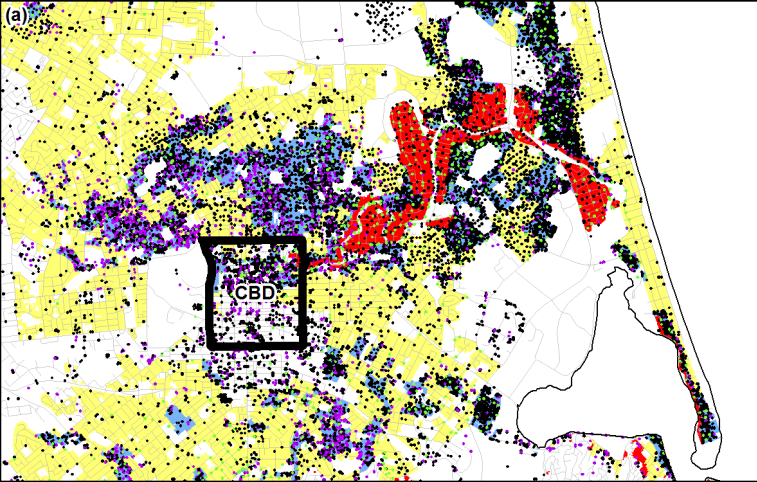
\includegraphics[width=1\textwidth]{images/Contexte/cgd.png}
%     % \caption{Visualisation des résultats de la base de données de Canterbury \cite{scott2015benefits}.}
%     \label{fig:canterbury}
% \end{figure}

% %............................

% \paragraph{}
% L'Afrique ne fait pas exception à la liste des multiples endroits ayant adopté l'idée
% de concevoir des bases de données géotechniques.
% Par exemple, celle de la ville de Tunis (Tunisie) est orientée vers la cartographie géotechnique.
% \par
% Le modèle choisi a permis, après une analyse
% pré1iminaire très importante, une description globale et
% totale de toutes les données géologiques et géotechniques collectées sur le site de Tunis. Il
% assure, de plus, une indépendance physique et logique, un partage des données (une même donnée accessible  
% par plusieurs programmes), une non-redondance des données, une grande facilité des relations
% entre fichiers indépendants, une intégrité (validité)
% totale des données. 
% \textit{S'y ajoutent une souplesse remarquable d'interrogation de TUNIS-DATA-BANK
% assurée par l'emploi d'un langage d'interrogation spécifique et l'utilisation des opérateurs et des connecteurs
% logiques, une automatisation totale des tâches de la
% phase de la manipulation de la base de données et une
% sécurité totale des fichiers.}
% \cite{mongereau1988conception}

% %..................
% \paragraph{} 
% Parmi les BDD géotechniques gouvernementales (Figure:\ref{fig:BDG}), la Base de Données Géotechniques
% (BDG) du gouvernement canadien, plus précisément le
% ministère des transports du Québec, et le "Geotechnical Web Mapping App" (Figure:\ref{fig:wash}) se font remarquer
% de par leur simplicité et leur efficacité. Ces deux systèmes présentent les sondages, les forages ainsi que les 
% propriétés des sols et des roches dans plusieurs zones de ces deux pays.
% Un webmap est utilisé pour faciliter la visualisation de ces données.
% De plus, le résultat de chaque étude est mis à la disposition du public
% via un lien PDF.

% \begin{figure}[t]
%     \centering
%     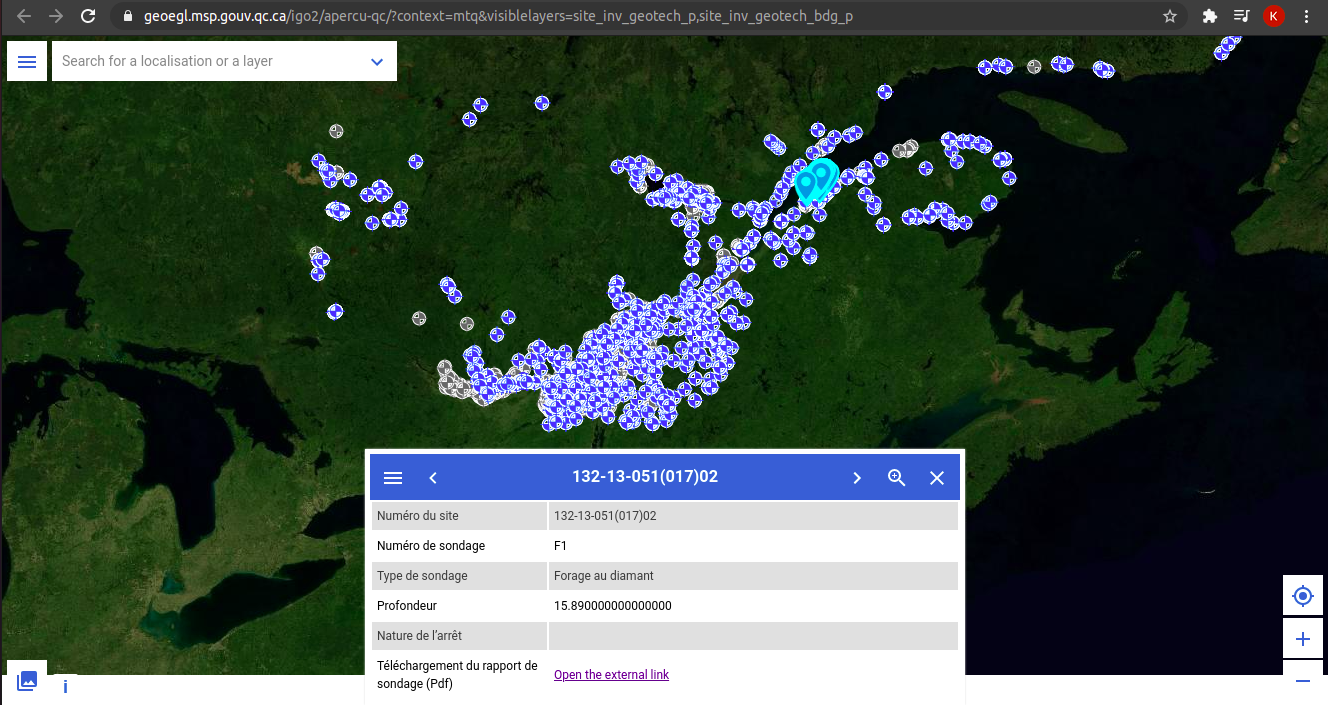
\includegraphics[width=1\textwidth]{images/Contexte/bdg.png}
%     % \caption{Webmap de la BDG du gouvernement du Canada \cite{canadagov}}
%     \label{fig:BDG}
% \end{figure}
% \begin{figure}[t]
%     \centering
%     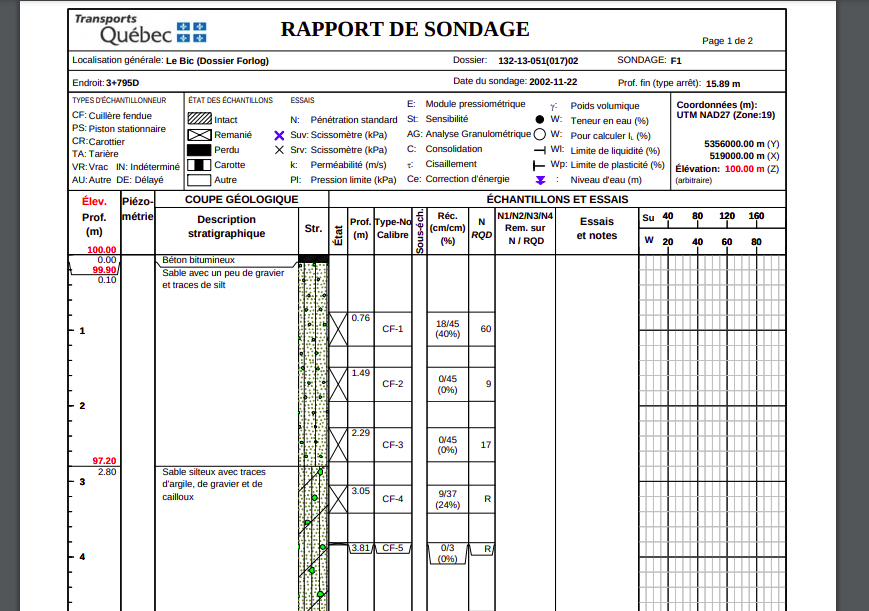
\includegraphics[width=1\textwidth]{images/Contexte/pdf_bdg.png}
%     \caption{PDF d'un rapport de sondage de la BDG du gouvernement du Canada \cite{linkpdfcanada}}
%     \label{fig:PDF_BDG}
% \end{figure}
% \begin{figure}[t]
%     \centering
%     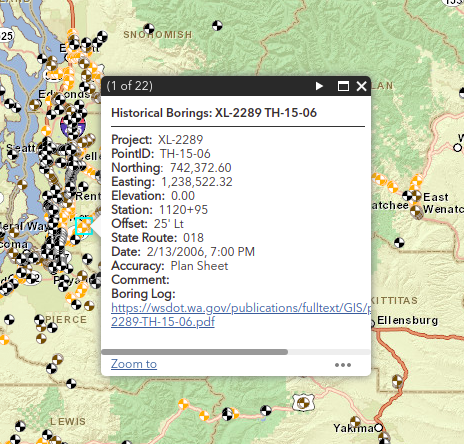
\includegraphics[width=1\textwidth]{images/Contexte/wash.png}
%     \caption{Information sur une étude spécifique dans le Geotechnical Web Mapping App \cite{map1}}
%     \label{fig:wash}
% \end{figure}

% \paragraph{}
% L’implémentation de tous ces SIG par des organismes internationaux résulte à des données considérées 
% comme étant le système d’archivage officiel dans leur domaine de spécialité.
% Le rythme de migration de ces données dans le SIG Web connait une croissance exponentielle. 
% Quelques exemples sont donnés dans le tableau \ref{tab:someBDD}.
% \par
% Avec son mouvement vers le cloud et sur le Web, son intégration à l'information 
% en temps réel via l'Internet des objets, le SIG est devenu une plateforme 
% pertinente pour presque toutes les activités humaines - un système nerveux de 
% la planète. Alors que notre pays est confronté au problèmes de gestion et de vulgarisation 
% des données géotechiques, les SIG joueront un rôle de plus 
% en plus important et 
% fourniront un moyen de communiquer des solutions en utilisant le langage commun de 
% la cartographie.

% \par    
% \begin{table}
%         \centering
%         \begin{tabular}{|p{0.40\linewidth}|p{0.60\linewidth}|}
%         \hline
%                 \textbf{BDD} & \textbf{Fonctions} \\
%                 \hline
%                     British Geological Survey (BGS) créée par le
%                     Royaume-Uni&
%                     Fournisseur de données, 
%                     d’informations et de connaissances 
%                     géoscientifiques objectives britannique
%                          \\
%                 \hline
%                     SERNAGEOMIN (Figure:\ref{fig:chili}) créée par le
%                     Gouvernement du Chili&
%                     Génération 
%                     d'informations géologiques sur le territoire 
%                     chilien, ses dangers géologiques et sa mise 
%                     à disposition des citoyens
%                          \\
%                 \hline 
%                     La base de données géotechniques de Canterbury (CGD) créée par le
%                     Gouvernement de la Nouvelle Zélande&
%                     Génération 
%                     d'informations géologiques sur le territoire 
%                     chilien, ses dangers géologiques et sa mise 
%                     à disposition des citoyens
%                         \\
%                 \hline 
%                     DBG créée par
%                     Ministère des transports du Québec&
%                     - Présentaion des sondages
%                     - Présentaion des forages sous forme schématique
%                     - Présentaion des propriétés des sols et des roches
%                     - Présentaion de la qualité de l’eau souterraine
%                         \\
%                 \hline 
%                 GISOS créée par
%                 trois organismes: BRGM, INERIS, INPL-LAEGO&
%                     - Accès facile aux informations sur les forages
%                     - Accès aux mouvements de terrain
%                     - Accès aux mesures topographiques
%                     - Accès aux essais au laboratoire
%                         \\
%                 \hline 
%                 Base de données géotechniques, géodésiques
%                  et géophysiques dans les argiles du Trièves créée par
%                  le conseil général de l'Isère&
%                         -Mise à disposition des utilisateurs potentiels, scientifiques ou opérationnels des informations
%                         géotechniques, géodésiques et géophysiques.
%                        \\
%                 \hline 
%                 SIGPEG
%                 et géophysiques dans les argiles du Trièves&
%                         - Accès aux informations sur les données
%                         cartographiques, géophysiques, géotechniques, sur les puits forés
%                             \\
%                 \hline 
%         \end{tabular}
%         \caption{Présentation de quelques BDD géotechniques dans le monde} \label{tab:someBDD}
% \end{table}
% \par

% \begin{figure}[t]
%     \centering
%     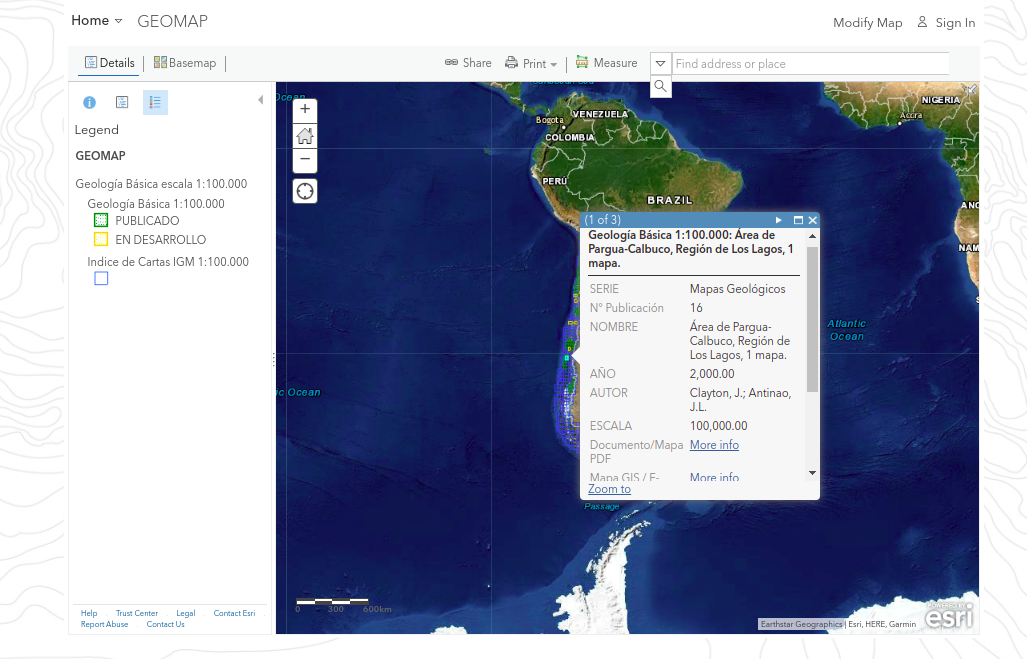
\includegraphics[width=1\textwidth]{images/Contexte/chili.png}
%     \caption{Webmap de SERNAGEOMIN \cite{map2}}
%     \label{fig:chili}
% \end{figure}

        \subsection{Avantages d'un Système de gestion des Informations Géotechniques}
            \paragraph{}
Les avantages apportés par le développement d'un systeme d'information géotechique
sont multiples.
L'un des plus important est la facilité avec laquelle les données 
peuvent être visualisées, filtrées et manipulées.
De plus, le risque de trouver  des informations inexactes est considérablement
réduite grâce aux protrocoles du métier, à la validation des données et aux processus
de contrôle approfondis.

\textit{ Une 
étude réalisée par Goldin et al.,
(2008) a montré qu'en moyenne 1,24\% des entrées de données dans Excel 
sont saisies de manière incorrecte; l'erreur alors
composés chaque fois que les données sont réintroduites. La mise en place 
«à entrée unique» d’une base de données bien conçue réduit les erreurs de 
transcription humaine, source majeure d’inexactitude pour les entreprises
traitant de grandes quantités de données géotechniques.}
\cite{keen2015development}
\paragraph{}
Ce projet peut aussi être
conçu comme un référentiel consultable pour le partage d'informations 
géotechniques existantes et nouvelles.
Il sera un outil de soutien pour les autorisations de construction délivré par l'État haïtien.
\paragraph{}
\par
Ces données peuvent également être utilisées à des fins plus stratégiques telles que l'aide à la
relèvement en cas de futures catastrophes naturelles.
Elles peuvent être utiles pour  l'élaboration des processus réglementaires.
La vaste base de données géotechniques
combinée à d'autres ensembles de données permettra un examen et une modélisation approfondis du terrain
et la performance de l'infrastructure à construire. 
\par
Les leçons tirées de ces analyses peuvent être appliquées pour
améliorer la résilience et également utilisé pour éclairer les 
décisions de politique réglementaire dans d'autres domaines en Haïti.
\paragraph{}
En plus du partage des données, une base de données géotechniques
offre les avantages suivants:
\begin{itemize}
    \item Diminution des coûts de maintenance des données géotechiques
    \item Les professionels peuvent accéder plus facilement aux informations géotechniques
    fournis par d'autres, économisant certains frais d'enquête
    \item Des évaluations de haut niveau peuvent être effectuées pour des
    projets utilisant des informations de la zone environnante pour
    mieux renseigner le profil géotechnique avant de s'engager à
    études plus détaillées
    \item Les données d'une zone peuvent être
    accessible pour servir de référence pour le terrain  dans des contextes géologiques similaires
    \item Les fournisseurs d'infrastructure peuvent être mieux informés
    et mieux cibler les zones les plus vulnérables , et, suite à un événement, optimiser les réparations
    \item  Les données souterraines peuvent être fournies aux autorités réglementaires
    et les décideurs pour leur permettre de prendre
    les décisions d'aménagement du territoire et déterminer la pertinence
    des stratégies et solutions d'investissement
    \item  Les entrepreneurs spécialisés peuvent évaluer les opportunités
    investir dans des équipements spécialisés et améliorer les sols de construction
    \item Améliorer la modélisation de sinistres catastrophes pour les assurances et
    la gestion des dangers. Cela facilerait la réalisation de scénario approprié
\end{itemize}

\paragraph{}
Cette base de données géotechiques permet aussi à la communauté
scientifique d'avoir accès à certaines données qui normalement seraient 
hosrs de porté cause des contraintes budgétaires. La recherche devient alors plus 
facile dans le domaine de la géotechique en Haïti.


\paragraph{}
Étant donné que cet outil n'existe pas encore
en Haïti, l'ampleur de ce projet fait donc surface.
D'où l'implémentation qui suit.


\par    
\begin{table}
        \centering
        \begin{tabular}{|p{0.10\linewidth}|p{0.80\linewidth}|}
        \hline
                \textbf{ } & \textbf{Avantages} \\
                \hline
                    1 &
                    Réduction du risque de trouver des informations inexactes
                    \\
                \hline 
                    2 &
                    Pas de duplication des données
                    \\
                \hline 
                    3 &
                    Création d'un référentiel consultable pour le partage d’informations géotechniques
                    \\
                \hline 
                    4 &
                    Diminution des coûts de maintenance des données géotechiques
                    \\
                \hline 
                    5 &
                    Disponibilité des données géotechiques
                    \\
                \hline 
                    6 &
                    Sécurité des données géotechiques
                    \\
                \hline 
                    7 &
                    Faciliter les prises de décisions d’aménagement du territoire 
                    et déterminer la pertinence des stratégies et solutions d’investissement
                    \\
                \hline 
                    8 &
                    Améliorer la modélisation de sinistres catastrophes pour les assurances
                    \\
            \hline 
        \end{tabular}
        \caption{Listes de quelques avantages d'une base de données géotechniques} \label{tab:avantages}
\end{table}
\par

    \section{La solution proposée}
        \paragraph{}
        Face aux différents problèmes que l'on constate, la solution que l'on propose est la suivante:
        Il s'agit de créer une base de données permettant de présenter et référencer l’ensemble des 
        données géotechniques dans un Système d’Information Géographique.
    
        \subsection{Les apports de cette solution}
            Ce sera une base de données relationnelle liée a une application web
            \footnote{Le choix des technologies est justifié dans le chapitre 3} 
            qui va assurer:
            \begin{itemize}
                \item la disponibilité des données
                \item l'intégrité des données
                \item la confidentialité
                \item la non répudiation
                \item un filtrage optimal des données
                \item la visualisation des données via un webmap
                \item l'accès aux données par les professionnels et universitaires
                \item la diminution des coûts liés a la gestion des données
                \item la sécurité des données face aux catastrophes humaines (sabotage)
                \item la sécurité des données face aux catastrophes naturelles (incendie, tremblement de terre, etc)
                \item l'exploitation des données par des entreprises et l'État pour les prises de décisions
                \item l'amélioration des modèles liés aux domaines géotechniques
                \item facilitation des recherches académiques et scientifique dans le domaine géotechique
                \item ...
            \end{itemize}
        \subsection{Analyse des risques}
        Les risques liés à la réalisation de ce projet sont multiples.
        \paragraph{Risques sur le plan social :}
        \begin{itemize}
            \item \textbf{Les entreprises :}
            L'enjeu pricipal est de convaincre les entreprises à accepter de rendre publiques des 
            données qui non seulement ont toujours été privées mais aussi qui coûtent chers. 
            Qu'auront-il à gagner en faisant ce geste ? 
            Comment arriver à les motiver à faire un tel sacrifice ?
            \item \textbf{Les visiteurs :}
            De plus il faut arriver à inciter les professionels et les etudiants à
            visiter la plateforme. Un flux d'activités important montrera l'intéret accordé à l'outil.
        \end{itemize}
        
        \paragraph{Solution :}
        La motivation des entreprises sera issue des avantages que l'on leur offrira et de l'ambiance
        scientique dans laquelle ils se trouveront en utilisant l'outil. 
        Tout un concepte sera mis en oeuvre : celui  \textbf{de science participative}.
        Il s'agit de créer une communauté dans laquelle chacun est libre d'aporter sa contribution 
        à la réussite du projet. Les entreprises seront en symbiose au gré des ingénieurs, étudiants 
        et autres entreprises(banques, assurances, l'État, ...) en quête de données géotechniques.
        Ce sera un environnment de partage entre scientifiques. Une campagne de sensibilisation à l'utilisation 
        de l'outil est prévue. Son importance est capitale dans le processus de motivation dans laquelle 
        tout entrepriseet tout utilisateur doit se retrouver.
        \par
        Pour l'ingénieur, ce sera un outil d'aide à la décision. Il peut optimiser son travail en exploitant
        les données de la plateforme. Ainsi, cela évitra aux particuliers désirant réaliser une construction
        d'être soumis aux lourdes contraintes budgétaires qu'implique une étude de sol.
        \par
        Pour l'étudiant, ce sera un outil de travail lui permettant de s'exercer avec des données réelles 
        et le préparant pour la vie profosionnelle qui l'attend.
        \par
        Pour l'entreprise, ce sera un outil lui permettant d'evaluer les risques d'un investissement. Par 
        exemple une banque peut s'appuyer sur ces données pour savoir si un prêt pour une construction dans une zone
        est risqué ou pas.

        \paragraph{Risques sur le plan technique :}
        \begin{itemize}
            \item \textbf{Réalisation d'un système trop encombrant :}
            Un utilisateur peut se perdre facilement dans un système encombrant. Il convient de le mettre dans un environnment
            pour il pourra facilement naviguer. L'expérience utilisateur (UX) est un point essentiel sur lequel on doit s'attarder.
            \item \textbf{Ne pas utiliser les technologies appropriées :}
            L'analyse des besoins et l'étude de la faisabilité conduisent au choix des téchnologies adéquates pour la réalisation
            du système. Ces choix seront justifiées et adaptés à l'outil. 
            Il s'agit aussi de ne pas réinventer la roue mais de tirer avantage de l'existant tout en réalisant 
            un système adapté à Haïti.
        \end{itemize}
        \paragraph{Solution}
        Le processus UX est global, il ne s’agit pas d’une compétence isolée mais d’une nouvelle 
        démarche qui intègre un nouveau membre de l’équipe projet : l’utilisateur. \cite{Schaudel2020}
        Il s'agira de co-construire l'interface avec l'utilisateur. On lui offre d'abord un espace simple et attrant
        tout en étant à l'écoute de ses feedbacks. Dans ce sens, une version Beta de l'application sera lancé et sera prête
        à être améliorée en fonction des demandes des utilisateurs.
        \par


    \section{Cheminement de la solution}
        \subsection{Implémentation d'une BDD géotechniques}
            \subsubsection{Numérisation des données}
                \par
Au cours de la première étape, des données seront recueillies à 
travers diverses instances, principalement l'URGéo ainsi que d'autres partenaires. 
Enregistrées sous divers formats(papiers, CSV, PDF entre autres), 
ces données seront par la suite normalisées puis numérisées. En 
effet, une structure uniforme devra être imposée afin de satisfaire la 
compréhension de tout particulier et le partage de ces données.
Cette étape a rapport à la standardisation des données et aux protocoles adoptés.
            \subsubsection{Intégration de ces données dans une BDD}
                \par
Évidemment, une simple numérisation ne changerait point grand chose 
si les données restent stockées sur des disques comme à l'ancienne. Ainsi, 
la normalisation ayant apporté un standard et une uniformité au sein des informations 
enregistrées, ces dernières pourront parfaitement être intégrées dans 
une base de données créée à cette fin. Une fois implémentée, cette 
base pourra héberger toutes les informations géotechniques relatives 
à une analyse effectuée par l'une des instances concernées. Plus 
explicitement, l'URGéo pourra enregistrer les résultats obtenus lors 
d'un forage, en alimentant la BDD tout en respectant les critères de 
standardisation.
\paragraph{}
Bien qu'efficace, cette BDD géotechniques reste un concept assez 
abstrait pour un concerné direct qui ne verra aucune différence 
entre ce nouveau format et les fichiers auxquels il était 
précédemment habitué.
        \subsection{Utilisation d'un SIG}
            \subsubsection{Connection de la carte d'Haïti et de la BDD}
                \par
Comme réalisé dans différents pays à travers le monde, la prochaine 
étape consistera à utiliser un Système d'Information Géographique (SIG) 
capable de faciliter l'interprétation scientifique de ces données. 
Les SIG permettent aux utilisateurs de créer leurs propres couches de cartes 
afin de résoudre des problèmes concrets. Ils ont également évolué ces dernières années pour 
devenir un moyen de partage de données et de collaboration, inspirant une 
vision qui devient aujourd’hui une réalité. Une base de données qui 
couvre pratiquement tous les sujets; dans le cas présent, ce sera la géotechnique. 
Une fois le SIG lié à la base, tout intéressé pourra accéder aux informations 
enregistrées, dans un format plus conventionnel. Cela facilitera la visualisation des données. 
Dans le cadre de ce projet, il 
pourra trouver les résultats des tests effectuées au niveau d'une zone précise.
            \subsubsection{Utilisation de fonds de carte}
                \par
Une fois les informations accessibles, l'interprétation devient 
plus évidente; ce qui peut, pourtant, s'avérer insuffisant. Par 
ailleurs, des images relatives au contexte recherché par le scientifique 
le mettra dans un environnement avec le maximum de détails. De ce fait, 
différents fonds de carte seront mis 
à la disposition de ce dernier, facilitant sa manipulation des données. 
L'ingénieur civil voulant faire des études en hydraulique pourra ainsi 
interprêter les données relatives à son domaine en sélectionnant 
le fond le carte qui lui convient.
\paragraph{}
Désormais, tout particulier pourra accéder aux données de la BDD 
géotechnique en se référant à son domaine d'étude. Néanmoins, jusque-là,
l'accès direct aux données de la base demandera l'intervention d'un 
expert en base de données.
        \subsection{Visualisation des données} 
            \subsubsection{Implémentation d'un UI intégrant un webmap}
                \par
Finalement, la dernière étape consistera à mettre à la disposition 
de nos utilisateurs finaux un interface adéquat et facilement 
accessible, leur permettant ainsi d'interagir avec la BDD. Grâce 
à cela, un administrateur pourra directement ajouter, afficher, modifier ou supprimer 
des informations sans avoir à contacter un expert en informatique.
Quant aux simples visiteurs, ils auront la possibilité de visualiter les données sur une carte. 
Ces données vont permettre aux utilisateurs(ingénieurs, étudiants, etc) de prendre des décisions, 
d’analyser des situations précises, ou encore de donner des alertes par rapport à des évènements précis.
\par
En effet, l'autonomie de tous les utilisateurs sans formation préliminaire 
traduira la performance de l'application. L'expérience utilisateur n'est pas anodin dans 
le développement d'un tel système.
            \subsubsection{Publication de l'interface}
                \par
Quelle serait l'utilité d'une application de cette envergure 
si sa portabilité n'était pas prise en compte ? - Aucune. Par 
conséquent, son déploiement dans le cloud relèvera d'un processus incontournable 
afin de la mettre à la disposition de tous les intéressés. Désormais, 
n'importe qui aura la possibilité d'accéder au portail web sans 
installation préalable. Néanmoins, pour une question de sécurité, 
certaines fonctionnalités exigeront à l'utilisateur/administrateur une authentification.
        \begin{figure}[t]
            \centering
            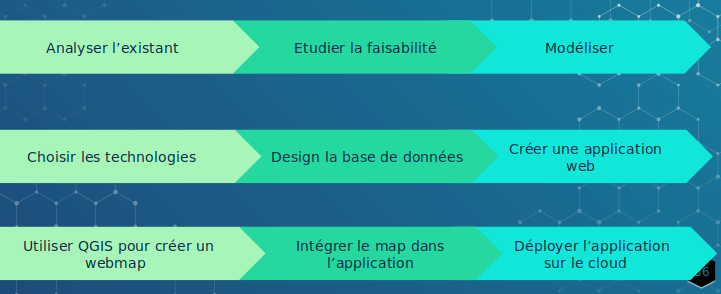
\includegraphics[width=1\textwidth]{images/Contexte/evolution_projetGIS.png}
            \caption{Cheminement de la solution}
        \end{figure}

    \section{Perspective de réalisation}
        \par
Étant plus que pragmatiques, nous ne nous limiterons pas à proposer 
uniquement une solution théorique. Nous mettrons la main à la pâte afin
de donner des résultats palpables et fonctionnels.
\par
Pour ce faire, nous définissons un cheminement, un ensemble d'étapes à 
respecter pour aboutir à un résultat optimal au moindre coût.
Ce cursus comprend cinq grandes étapes: 

\begin{itemize}
    \item \textbf{L'initialisation du projet: }
    Cette étape marque le début de notre long parcours et aura comme principaux
    objets la prise de connaissance du problème (dans le CDC) et l'identification des voeux
    l'URGéo.
    \item \textbf{Planification: }
    Tout grand projet digne de ce nom doit être planifié. C'est au cours de cette étape
    que l'état de l'art sera traité pour prendre connaissance de l'existant et s'inspirer des travaux
    similaires déjà réalisés. Puis vient la phase de l'analyse, de l'évaluation des coûts du projet, 
    du choix  de l'architecture, des modèles,
    ainsi des technologies et des méthodes que l'on aura à utiliser.
    \item \textbf{Exécution: }
    L'essence de cette étape se trouve dans la réalisation même du projet, que ce soit en matière de base de 
    données ou de programmation.
    \item \textbf{Monitoring et contrôle: }
    Ici il s'agit d'effectuer des tests sur la qualité du produit final et et de vérifier si on a atteint le 
    résultat escompté. Notons que cette partie pourra se faire en parallèle avec l'éxécution, en faisant de 
    l'intégration continue.
    \item \textbf{Fermeture: }
    Enfin, on aboutit à la clôture du projet apres déploiement et une potentielle période de maintenance.


\end{itemize}   


\chapter{Analyse des besoins}
        Nous débutons la conception de notre système en analysant la
situation pour prendre note des différentes contraintes, des risques
et tout autre élément pertinent dans le but de satisfaire l'intégralité
des besoins de l'URGéo.  Nous sommes déjà imbus du contexte de développement
du système, par conséquent, nous allons, dans cette partie, nous concentrer
sur les besoins et les contraintes de l'application.
\section{Besoins et contraintes}
        Il s'agit de la conception d'une base de données géotechniques et d'une
        application web permettant de visualiser cesdites données. Définissons
        d'abord tous les besoins des différents utilisateurs du système.
        \subsubsection{Identification des acteurs du système}
        Pour connaître les différents besoins des utilisateurs, nous devons
        avant tout relever la liste des différents utilisateurs eux-mêmes.
        Nombreux sont ceux qui auront à utiliser le système. Nous appellerons ces différents
        utilisateurs  les \textbf{acteurs} du système.
        \par
        L'application est disponible pour tout le monde notamment les
        professionnels en géosciences, les ingénieurs, les étudiants, les banques, les 
        compagnies d'assurance, etc.
        Ces acteurs sont divisés en trois (3) catégories:
        \begin{itemize} 
                \item \textbf{les visiteurs: }
                Un visiteur est un utilisateur externe qui se rend sur l'application pour rechercher et visualiser
                les données mises disponibles par l'URGéo et les instances associées. 
              
                \item \textbf{les administrateurs: }
                Un administrateur est un utilisateur interne capable d'interagir directement avec les données. 
                Il a pour principal rôle la gestion des data 
                liés aux différents résultats géotechniques. Tout au long du document, on entendra par data:
                \begin{itemize}
                        \item Les résultats des essais 
                        \item Les fonds de carte
                \end{itemize}
                Il est obligatoire pour lui de s'authentifier pour pouvoir 
                effectuer certaines actions sur le système. Seront administrateurs, toute personne désignée par l'URGéo
                ou les partenaires de l'URGéo. Le plus souvent, il s'agira des stagiares responsables de l'entrée 
                des données.

                \item \textbf{les superadmins: }
                Un super-administrateur est un super utilisateur. Détenant un rôle particulièrement sensible,
                il est obligatoire pour lui de s'authentifier pour y accéder. Ses droits sont particulièrement orientés 
                vers la gestion des ressources du système. Il peut ainsi manipuler les informations relatives aux 
                différents utilisateurs et garder un trace des trafics effectués au sein de l'application.
                 Seront superadmins, toute personne désignée par l'URGéo.
            \end{itemize}   
        \subsubsection{Besoins des différents utilisateurs}
        Étant donné que l'on a deux types d'utilisateurs internes avec des privilèges différents,
        le système doit impérativement comporter un mode de gestion des utilisateurs et des droits d'accès.
        \paragraph{Le visiteur}
        Le visiteur a à sa disposition une carte d'Haïti marquée aux différents endroits où des tests 
        géotechniques ont été réalisés.
        À n'importe quel moment, il peut décider d'effectuer une recherche par mot clé et s'attend
        à ce que le résultat de sa recherche s'affiche sur la carte. Il a aussi l'option de l'afficher sous la forme
        d'une liste qu'il peut filtrer selon son choix. Cette dernière peut être téléchargée sous format CSV.
        En support aux informations spécifiques à un test se trouvant à un endroit bien précis sur la carte,
        le visiteur a aussi l'accès au résultat du test se trouvant dans un fichier PDF qu'il peut télécharger.
        \par
        Aussi, plusieurs fonds de carte seront disponibles permettant au visiteur d'adapter le résultat de ses recherches
        au contexte idéal (topographie, hydraulique,... )
        \par
        Le visiteur peut aussi décider de lire, de commenter ou de laisser un message (de manière anonyme ou pas) 
        sur le forum dédié à l'application.
        \paragraph{L'administrateur}
        Un administrateur ne peut exister sans appartenir à une institution su système. Avant tout, il peut réaliser 
        toutes les actions d'un visiteur. De plus, après s'être authentifié au moyen de 
        son adresse électronique et de son mot de passe, il peut interagir directement avec la base de données. En cas 
        d'oubli de son mot de passe, le système lui envoie un lien de réinitialisation de mot de passe à son email.
        Pour jouer son rôle d'administrateur, il est redirigé vers \textit{l'interface de l'administrateur}. 
        Dans ce module, l'administrateur peut:
        \begin{itemize}
                \item \textbf{Ajouter un test: }
                Il s'agit de rentrer les informations relatives à un test pour l'ajouter dans la base de données.
                Ces informations sont de types différents (nom:texte, identifiant:entier, date du test:date, types
                de test:entier, date d'enregistrement:date, etc\footnote{Les différents champs et leur type seront 
                détaillés dans l'étude des diagrammes à la fin du chapitre} )
                \item \textbf{Modifier un test: }
                Si pour une raison ou pour une autre un test doit être modifié, l'administrateur est en
                mesure de le faire après s'être authentifié. Un message lui sera affiché à l'écran dépendemment 
                de la réussite ou de l'échec de son action. 
                \item \textbf{Supprimer un test: }
                La suppression d'un test est aussi possible. Un message de confirmation précède la validation
                de l'exécution de cette action car elle est irréversible.
        \end{itemize}
        \par
        À noter qu'il ne peut s'aventurer à modifier ou supprimer un test qui n'avait pas été directement 
        ajouté par un administrateur appartenant à la même institution. De plus, si l'URGéo juge que le commentaire d'un visiteur doit être supprimé,
        l'administrateur est apte à réaliser cela.
        \par
        Chaque action effectuée par un administrateur sera enregistrée automatiquement pour permettre la traçabilité
        et la non-répudiation\footnote{On abordera cette partie dans la section sécurité du chapitre 3.}.
        Ainsi, un module permettant de visualiser uniquement les logs\footnote{Historique des actions effectuées sur un 
        système informatique.} du système. Par conséquent, on peut savoir
        la date et l'heure précise où un administrateur ouvre une session, affiche, ajoute, modifie ou supprime une donnée.
        Nul utilisateur ne pourra altérer ces donnéees.
        \par

        \paragraph{Le superadmin}
        Il s'agit là de l'utilisateur de plus haute hiérarchie de notre application. Certes, il est libre 
        d'utiliser l'application comme un simple visiteur. De plus, après s'être authentifié au moyen de 
        son adresse électronique et de son mot de passe, il peut avoir accès tant aux données relatives aux
        différents utilisateurs de son institution qu'au trafic des différentes données en circulation. Il 
        pourra ainsi visionner les statistiques relatives au bien fondé de la plateforme.
        Dans ce module, le superadmin peut:
        \begin{itemize}
                \item \textbf{Ajouter un utilisateur: }
                Il s'agit de rentrer les informations relatives à un utilisateur pour l'ajouter dans la base de données.
                Ces informations sont de types différents (nom:texte, prénom identifiant:entier, type d'utilisateur, 
                etc\footnote{Les différents champs et leur type seront 
                détaillés dans l'étude des diagrammes à la fin du chapitre} )
                \item \textbf{Modifier un utilisateur: }
                Si pour une raison ou pour une autre les informations d'un utilisateur doivent être modifiées, le superadmin est en
                mesure de le faire après s'être authentifié. Un message lui sera affiché à l'écran dépendemment 
                de la réussite ou de l'échec de son action.
                \item \textbf{Activer ou désactiver un utilisateur: }
                Il s'agit d'autoriser ou non un administrateur à utiliser l'application.
                \item \textbf{Visionner la statistique des trafics effectués sur les données de son institution: }
                Un graphe statistique sera mis à sa disposition sans qu'il ne puisse le modifier personnellement.
        \end{itemize}
          

\par    
\begin{table}
        \centering
        \begin{tabular}{|p{0.21\linewidth}|p{0.54\linewidth}|p{0.33\linewidth}|}
        \hline
                \textbf{Utilisateurs} & \textbf{Besoins} & 
                \textbf{Contraintes}  \\
                \hline
                        Visiteur & 
                        \begin{itemize}
                                 \item[$\cdot$]  Cartographie d'Haïti
                                 \item[$\cdot$]  Fonds de carte
                                 \item[$\cdot$]  Recherches
                                 \item[$\cdot$]  Filtrage des donnéees
                                 \item[$\cdot$]  Téléchargement des résultats des tests
                                 \item[$\cdot$]  Navigation simple et attrayante
                        \end{itemize} & 
                        Accès au site à partir du lien \\
                \hline
                        Administrateur & 
                        \begin{itemize}
                                \item[$\cdot$]  Ajout de test
                                \item[$\cdot$]  Modification de test
                                \item[$\cdot$]  Suppression de test
                                \item[$\cdot$]  Suppression de commentaire
                        \end{itemize} & 
                        \begin{itemize}
                                \item[$\cdot$] Authentification 
                                \item[$\cdot$] Appartenance à une institution du système 
                        \end{itemize}
                         \\
                \hline
                        Superadmin & 
                        \begin{itemize}
                                \item[$\cdot$]  Affichage des logs
                                \item[$\cdot$]  Ajout d'administrateur
                                \item[$\cdot$]  Modification d'administrateur
                                \item[$\cdot$]  Activation d'administrateur
                                \item[$\cdot$]  Désactivation d'administrateur
                                \item[$\cdot$]  Accès à l'analyse des flux de l'application 
                        \end{itemize} & 
                        \begin{itemize}
                                \item[$\cdot$] Authentification 
                                \item[$\cdot$] Appartenance à une institution du système 
                        \end{itemize}
                         \\
                \hline  
        \end{tabular}
        \caption{Tableau des utilisateurs et de leurs besoins} \label{tab:sometab}
\end{table}
\par
                \lipsum[1]
        \section{Approche de travail}
        \subsection{Le génie logiciel}
        \textit{
                En 1995, une étude du Standish Group dressait un tableau accablant de la 
                conduite des projets informatiques. Reposant sur un échantillon 
                représentatif de 365 entreprises, totalisant 8 380 applications, 
                cette étude établissait que \cite{audibert2009uml} :
                \begin{itemize}
                        \item 16,2\% seulement des projets étaient conformes 
                        aux prévisions initiales,
                        \item 52,7\% avaient subi des dépassements en coût et délai d'un facteur 2 à 3 
                        avec diminution du nombre des fonctions offertes,
                        \item 31,1\% ont été purement abandonnés durant leur développement.
                \end{itemize}
        }
        \paragraph{}
        GéoTechMap doit faire partie de ces 16,2 \%. Pour ce faire, il ne faut surtout pas
        négliger l'importance du génie logiciel.
        \par
        Le génie logiciel est un domaine de de recherche qui a pour objectif
        d'optimiser le coût de développement d'un logiciel. De ce fait, notre
        travail en tant qu'ingénieurs est de nous occuper de l'architecture
        du logiciel, en l'occurence ses composants ainsi que ses mécanismes.
        La conception passe par plusieurs phases. Ainsi, on établie une approche
        de travail qui permettera de répondre aux besoins grandissants du système 
        que l'on va concevoir.
        \par
        À la suite de l'évaluation et de la documentation des besoins spécifiques
        de l'URGéo, des utilisateurs et des spécifications logiques et matérielles
        relatif au système, un plan a été dréssé:
        \begin{itemize}
                \item l'analyse des besoins,
                \item l'élaboration des spécifications,
                \item la conceptualisation,
                \item le développement,
                \item la phase de test,
                \item déploiement,
                \item vulgarisation,
                \item la maitenance
        \end{itemize}
        \paragraph{Un système de qualité}
        \paragraph{}
        Il s'agira d'offir un logiciel de qualité qui s'appuera sur différents facteurs.
        GéoTechMap rempli exactement les fonction escomptés spécifieés dans le 
        cahier des charges. La validité du système ne pourra être mis en doute.
        De plus, ce sera un une application fiable et robuste, pouvant facilement
        être combiné avec d'autres logiciels (choix de développement API). Dans le 
        Tableau \ref*{tab:facteurs}, figurent les differents facteurs sur lesquels reposent la qualité
        de GéoTechMap.

\par    
\begin{table}
        \centering
        \begin{tabular}{|p{0.20\linewidth}|p{0.80\linewidth}|}
        \hline
                \textbf{Facteurs} & \textbf{Détails} \\
                \hline
                Facilité d'emploi &
                facilité d'apprentissage, d'utilisation, de préparation des données, 
                d'interprétation des erreurs et de rattrapage en cas d'erreur d'utilisation.
                         \\
                \hline
                Validité&
                aptitude d'un produit logiciel à remplir exactement ses fonctions, 
                définies par le cahier des charges et les spécifications
                    \\
                \hline
                Fiabilité &
                aptitude d'un produit logiciel à fonctionner dans des conditions anormales.
                    \\
                \hline
                Réutilisabilité&
                aptitude d'un logiciel à être réutilisé, en tout ou en partie, dans de nouvelles applications.
                    \\
                \hline
                Compatibilité&
                facilité avec laquelle un logiciel peut être combiné avec d'autres logiciels.
                        \\
                \hline
                Efficacité&
                Utilisation optimale des ressources matérielles.
                        \\
                \hline
                Portabilité&
                facilité avec laquelle un logiciel peut être transféré sous différents environnements matériels et logiciels.
                        \\
                \hline
                Vérifiabilité&
                facilité de préparation des procédures de test.
                        \\
                \hline 
                Intégrité&
                aptitude d'un logiciel à protéger son code et ses données contre des accès non autorisés.
                        \\

                \hline 
        \end{tabular}
        \caption{Quelques facteurs sur lesquels reposent la qualité
        de GéoTechMap \cite{audibert2009uml}} \label{tab:facteurs}
\end{table}
\par

        \subsection{Le cycle de vie du logiciel}
        Ce cycle désigne les principales étapes de développement du logiciel.
        Le but de cette sécantation est de permettre la vérification du processus de déveeloppement.
        Il comprend le plus souvent les étapes suivantes :
        \begin{itemize}
                \item L'analyse des besoins et la faisabilité du projet
                \item La conception
                \item Le codage
                \item Les tests
                \item La documentation
                \item La mise en production
                \item La maintenance
        \end{itemize}
        Le cycle de vie peut être modélisé de plusieurs manières (Figure \ref{fig:methv} ).
        Nous utiliserons ici le modèle du cycle en V car demeure actuellement le cycle de vie le 
        plus connu et certainement le plus utilisé. 
        Il s'agit d'un modèle en cascade dans lequel le 
        développement des tests et du logiciel sont effectués 
        de manière synchrone \cite{audibert2009uml}.
        \begin{figure}[ht!]
                \centering
                \begin{subfigure}{.45\linewidth}
                    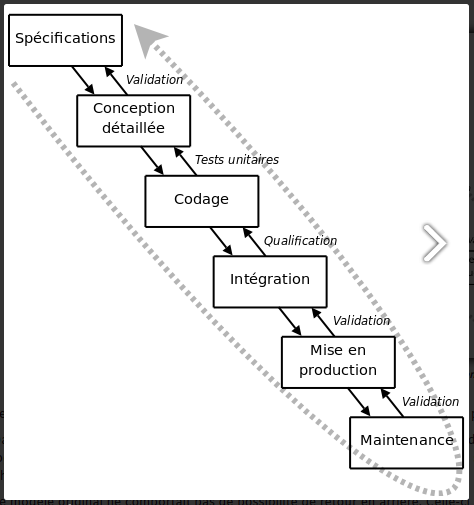
\includegraphics[scale=0.35]{images/Analyse_des_besoins/methcasc.png}
                    \caption{Modèle du cycle de vie en cascade}
                \end{subfigure}
                \hskip2em
                \begin{subfigure}{.45\linewidth}
                    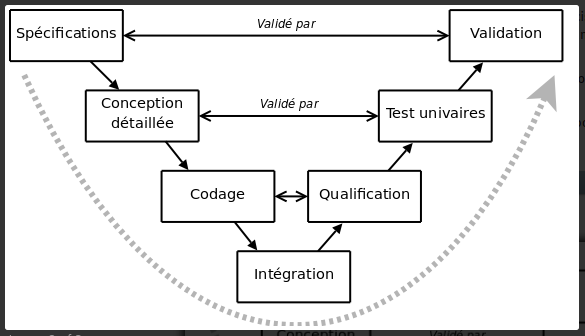
\includegraphics[scale=0.35]{images/Analyse_des_besoins/methv.png}
                    \caption{Modèle du cycle de vie en V}
                    \label{fig:methv}
                \end{subfigure}
               
            \end{figure}
           
       
        \section{Méthodologie}
        Pour la réalisation d'un système complexe, le traitement des problèmes doit se faire 
        de manière efficace. Les tâches lourdes serons divisées en de petites et assignées 
        à chaque membre de l'équipe  en fonction de ses aptitudes à les résoudre. En peu de mots,
        la méthodologie Agile et scrum est adoptée dans le cadre de ce projet.

        
        \paragraph{C’est quoi, la méthode Agile et Scrum ?}
        \paragraph{}
        \textit{Agile représente un ensemble de “méthodes et pratiques basées sur 
        les valeurs et les principes du Manifeste Agile”, qui repose entre autre sur 
        la collaboration, l’autonomie et des équipes pluri-disciplinaires}\cite{Littlefield2017}.
        \par
        La méthodologie Agile s'oppose généralement à la méthodologie traditionnelle waterfall (en cascade :
        \textit{dès qu'une étape du projet est terminée, l'équipe passe à l'étape suivante ; il n'y a pas (ou peu) 
        de retour en arrière}\cite{david2017}). Elle se veut plus souple 
        et adaptée, et place les besoins du client au centre des priorités du projet.
        \par
        \textit{Scrum est un framework qui est utilisé pour implémenter la méthode 
        Agile de développement et de gestion de projet}\cite{Littlefield2017}.

        \paragraph{}
        La méthode agile de gestion de projet et le framework Scrum est basé sur une méthode 
        itérative de livrables du produit. Au lieu d’attendre que le projet soit 100\% finalisé 
        pour le livrer au client, vous délivrez des tronçons “utilisables” du projet au cours du 
        temps. Vous éviterez ainsi de gaspiller des efforts en cas de nécessité de changement ou 
        de problème de communication. Au-delà de l’importance des itérations et des améliorations 
        pour le produit, Scrum s’attache également à améliorer le processus à chaque nouveau cycle.
        \paragraph{}
        Un projet Scrum peut être agencé de différentes manières mais sont toujours présents:
        \begin{itemize}
                \item Product Owner : Il représente les intérêts du client et à ce titre, il a 
                l’autorité pour définir les fonctionnalités du produit final. Dans notre cas, il s'agit de l'URGéo.
                \item Sprint : Scrum utilise des sprints comme intervalles de temps pendant lesquels l’équipe 
                va compléter un certain nombre de tâches. Chaque sprint se termine avec une Rétrospective, qui réunit 
                toute l’équipe afin de partager les retours d’expérience et discuter des améliorations possibles du 
                prochain sprint.
        \end{itemize}

        \paragraph{Pourquoi Agile et Scrum ?}
        \begin{itemize}
                \item Scrum est la méthode agile la plus éprouvée et la plus documentée.
                \item Contrairement à la méthode traditionnelle waterfall, l'approche Agile offre une plus 
        grande flexibilité et une meilleure visibilité dans la gestion du projet. 
                \item L'avantage majeur de l'approche Agile est sa flexibilité. Les changements du client et les imprévus 
        sont pris en compte et l'équipe projet peut réagir rapidement.
                \item Le client dispose d'une meilleure visibilité sur l'avancement du projet et peut ainsi l'ajuster 
                en fonction de ses besoins. Le contrôle qualité est permanent. Quant à l'équipe projet, elle peut 
                réagir rapidement aux demandes du client.\footnote{Qu'est-ce que la méthodologie Agile ? \url{https://www.planzone.fr/blog/quest-ce-que-la-methodologie-agile}}
        \end{itemize}
        
        
        

        \section{Structure modulaire}
                \lipsum[1]
        \section{Préparation des documents}
                

                \par
                Étant donnée que la majorité des rapports et résultats des tests sont 
                disponibles sous forme papier, la première étape a consisté à scanner les documents.
                Pour ce faire nous adoptons une protrocole: on assure la traçabilité de chaque 
                document les munissant d'une cartouche reprennant une série d'informations.
                Voici la liste des informations qui forme une cartouche:
                \begin{itemize}
                        \item \textbf{Lieu: }
                        Il s'agit de l'endroit où l'étude a été effectuée.
                        \item \textbf{Date: }
                        Il s'agit de la date à laquelle l'étude a été effectuée.
                        \item \textbf{Maître d'ouvrage: }
                        Il s'agit du client pour lequel l'étude est effectuée.
                        \item \textbf{Maître d'œuvre : }
                        Il s'agit de la personne ou l'entreprise chargée de l'étude.
                        \item \textbf{Réf Numéro Étude: }
                        Il s'agit d'un identifiant unique permettant de tracer une étude.
                \end{itemize}
                
\par    
\begin{table}
        \centering
        \begin{tabular}{|p{0.30\linewidth}|p{0.40\linewidth}|}
                \hline
                \textbf{Lieu} & Delmas \\
                \hline
                \textbf{Date} & Janvier 2020 \\
                \hline
                \textbf{Maître d'ouvrage} & Faculté Des Sciences \\
                \hline
                \textbf{Maître d'œuvre} & URGéo \\
                \hline
                \textbf{Réf Numéro Étude} & 1234 \\
                \hline
        \end{tabular}
        \caption{Exemple de cartouche sur un document d'étude géotechnique} \label{tab:example_cartouche}
\end{table}
\par

        \section{Modélisation avec UML}
        
\paragraph{Pourquoi modéliser ?}
\paragraph{}
La modélisation est le fait de représenter de manière abstraite et simplifiée
une entité du monde réel. Cette entité peut être un phénomène, un processus ou 
comme dans notre cas, un système. L'objectifif de la modélisation est de décrire
, d'analyser, d'expliquer ou de prévoir l'evolution de l'entité en question.
\paragraph{}
Le modèle est enfin indispensable pour assurer un bon niveau de qualité 
et une maintenance efficace. Le choix du modèle a donc une influence capitale 
sur les solutions obtenues.
\paragraph{UML}
\paragraph{}
Une image vaux mieux que milles mots.
Considérez que ce proverbe comme le résumé de l'origine
de la schématisation en langage de modlisation unifié.
Le langage UML (Unified Modeling Language) résume et visualise les 
systèmes de programmation orientés objet. UML est un langage de 
modélisation orienté objet, c’est-à-dire que toutes 
les entités modélisées sont des objets ou se rapportent à des 
objets \cite{conan}.

Son objectif est de créer un langage visuel commun dans le monde 
complexe du développement de logiciels. Il serait aussi comprehensible
par les professionnels et ceux qui veulent comprendre un système. 
\paragraph{}
Le Unified Modeling Language spécifie 14 types de 
diagrammes qui représentent la structure, le comportement et les interactions d’un système.
\subsection{Diagrammes des cas d'utilisation}
    \subsubsection{Cas général}
    \paragraph{}
    \begin{figure}
        \centering
        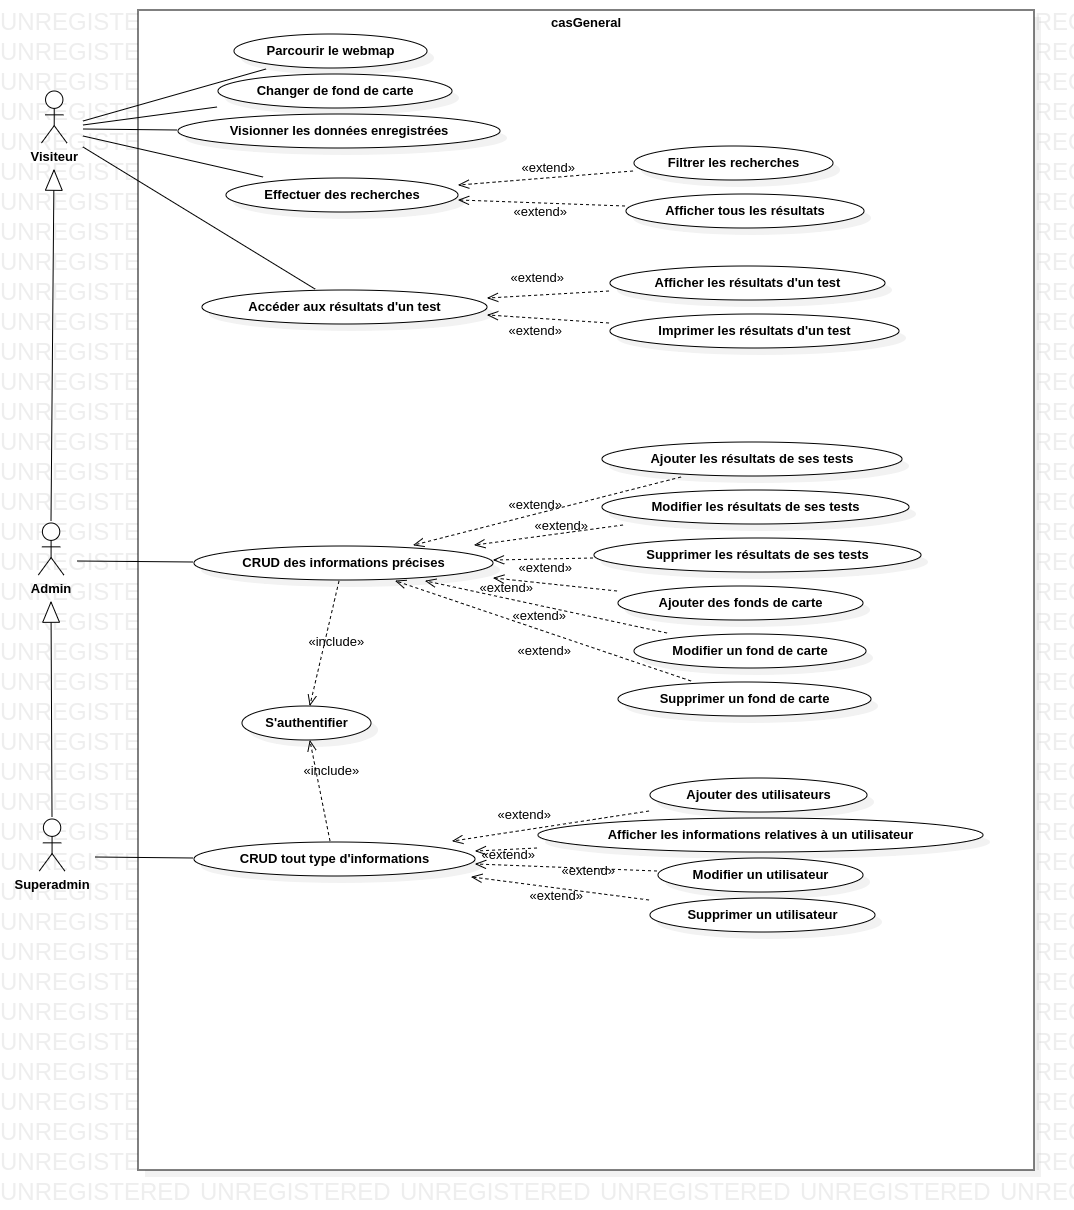
\includegraphics[width=1\textwidth]{images/Analyse_des_besoins/casGeneral.png}
        \caption{Diagramme des cas d'utilisation général}
    \end{figure}
    \par 
    Trois niveaux d'acteurs sont à considérer au sein du système: un visiteur, 
    un administrateur et un super administrateur. La hiérarchisation permet que 
    chaque niveau ait accès aux droits du niveau immédiatement inférieur. 
    De ce fait, un super administrateur est également un administrateur et 
    un visiteur en plus de son niveau direct. \par 
Pour commencer, le visiteur a des droits d'accès très restreints: \par 
\begin{itemize}
    \item Parcourir le webmap: Le visiteur peut voir l'ensemble des informations 
    géotechniques disponibles sur la carte.
    \item Changer de fond de carte: Afin de mieux illustrer le contexte marquant 
    l'intérêt du visiteur, une variété de fonds de carte est accessible sur le site. 
    Ainsi, l'utilisateur peut puiser dans le champs de choix qui lui sont proposés.
    \item Visionner les données enregistrées: En cliquant sur une légende précise, 
    le visiteur peut voir les données qui ont été préalablement enregistrées dans la base de données.
    \item Effectuer des recherches: Deux options s'offrent aux utilisateurs. Ces derniers 
    peuvent afficher tous les résultats au cours de la rechercherche, ou encore ils peuvent 
    se fixer des filtres capables de mieux limiter les plages des résultats.
    \item Accéder aux résultats d'un test: Une fois les résultats obtenus, le visiteur 
    peut soit simplement les afficher, soit les imprimer.
\end{itemize}

\paragraph{}
De son côté, l'\textbf{administrateur} s'occupe de la gestion des informations au sein de la base 
de données. En plus des droits de visiteur, ce type d'utilisateur peut:
\begin{itemize}
    \item Ajouter des informations géotechniques: L'admin peut ajouter des informations 
    dans la bdd, qui sont reflétées sur la carte. 
    \item Modifier les informations qu'il avait préalablement enregistrées: Il ne peut 
    modifier que les informations qu'il avait lui-même ajoutées.
    \item Supprimer les informations qu'il avait préalablement enregistrées: Tout comme il 
    en est pour la modification, il ne peut supprimer que les informations qu'il avait lui-même ajoutées.
    \item Ajouter un fond de carte
    \item Supprimer un fond de carte
\end{itemize}

\par 
Évidemment, aucune de ces actions ne saura avoir lieu tant que l'administrateur ne s'est pas authentifié.

En dernier lieu, le super administrateur joue surtout un rôle de gestionnaire en ressources 
humaines. Une fois authentifié, en plus des droits d'accès d'un simple administrateur, 
cet utiliateur peut:
\begin{itemize}
    \item Ajouter des utilisateurs
    \item Modifier les utilisateurs
    \item Afficher les informations relatives aux différents utilisateurs, pouvant 
    ainsi retracer toutes les actions posées par un utilisateur du système.
    \item Supprimer ou désactiver un utilisateur: La différence se fait remarquer 
    par le fait que le super admin peut supprimer complètement un utilisateur ainsi 
    que toutes les informations y relatives ou simplement désactiver le compte d'un 
    utilisateur sans, pour autant, éliminer ses données.
\end{itemize}

\subsubsection{Parcourir le Webmap}
    \paragraph{}
    \begin{figure}
        \centering
        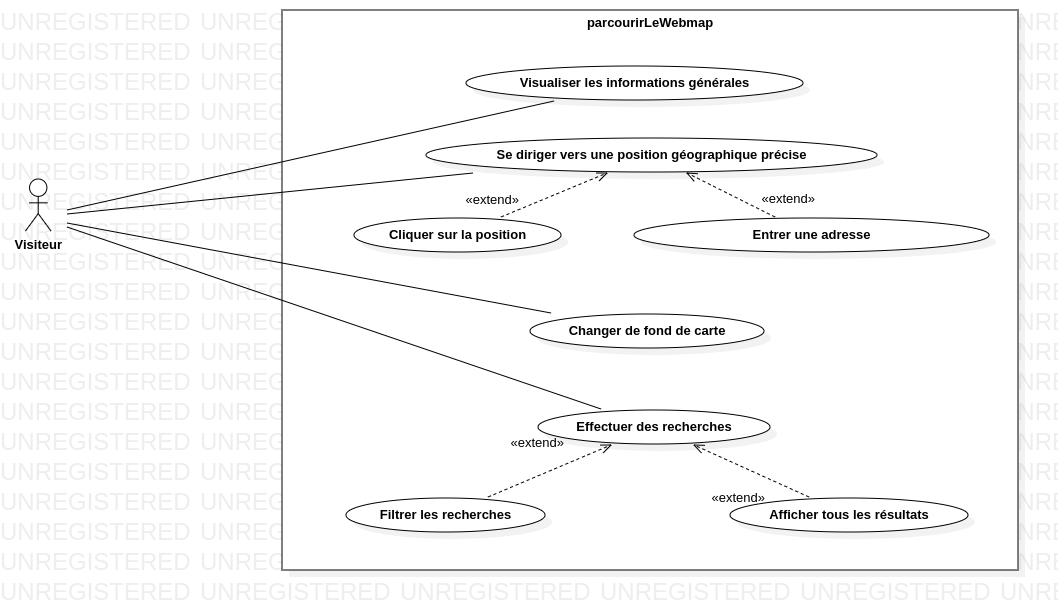
\includegraphics[width=1\textwidth]{images/Analyse_des_besoins/parcourirLeWeb.png}
        \caption{Diagramme du parcours du webmap}
    \end{figure}
\par 
Tout individu, concernés ou pas, par les informations fournies par 
le webmap peut parcourir l'application. Pour ce faire, aucune authentification 
n'est nécessaire au préalable. Lorsqu'un visiteur accède au site, il peut donc:
\begin{itemize}
    \item \textbf{Visualiser les informations générales:}
    Les informations sont disponibles sur une carte pouvant être interprétés
    par un particulier. Elles sont étiquetées sur les points géographiques respectives.
    De ce fait, il peut sélectionner une étiquette particulière afin d'avoir 
    accès à ces données, lui permettant de 
    \begin{itemize}
        \item Visualiser le fichier pdf
        \item Télécharger ce fichier
    \end{itemize}
    \par 
    À première vue, le visiteur ne voit que la carte remplie de 
    "pin[MPOKO JWENN TERME FRANCAIS A]" colorés relatifs à une légende 
    explicite pour la compréhension du visiteur. En plus des légendes, une liste 
    de wigdets facilitant la navigation de l'utilisateur.
    \item \textbf{Accéder à une position géographique précise}
    Toutes les informations étant disponibles, le visiteur peut choisir 
    de visualiser les données relatives à une position bien définies. Pour y accéder, il 
    peut:
    \begin{itemize}
        \item Cliquer directement sur la position géographique
        \item Entrer une adresse dans le champs y frelatif
    \end{itemize}
    \item \textbf{Changer de fond de carte}
    Chaque individu visite ce webmap dans un contexte personnel. Par 
    ailleurs, il peut changer le fond de la carte en fonction de 
    ses besoins. Ces images peuvent varier d'un point de vue hydraulique
    à un point de vue magmatique en passant par tous les fonds mis 
    à la disposition de l'utilisateur par les institutions.
    \item \textbf{Effectuer des recherches relatives aux essais}
    Grand nombre d'essais sont enregistrés sur la carte. Pour faciliter 
    la navigation, une possibilité de recherche est offerte. Dans ce cas,
    il peut donc:
    \begin{itemize}
        \item Afficher tous les résultats
        \item Filtrer les recherches 
    \end{itemize}
\end{itemize}

\subsubsection{Manipulation des données de la base}
    \paragraph{}
    \begin{figure}
        \centering
        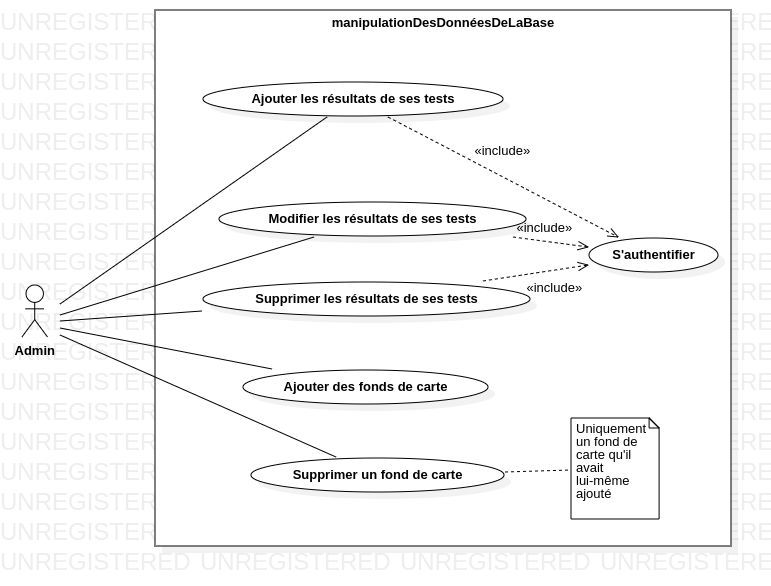
\includegraphics[width=1\textwidth]{images/Analyse_des_besoins/manipulationDesDonneesDeLaBase.png}
        \caption{Diagramme de la manipulation des données de la base}
    \end{figure}
    \par 
    Avant même que les données puissent être disponibles et interprétables 
    par un utilisateur, il faut qu'elles soient intégrées et manipulées continuellement. Le 
    seul utilisateur ayant habilité à faire de telles 
    actions est l'administrateur. Néanmoins, il ne peut manipuler que les informations 
    qu'il a lui-même insérées dans la base de données. Ces dernières étant sensibles, L'admin 
    doit s'authentifier avant d'avoir des droits d'accès à toute sorte de manipulation.

    \subsection{Diagramme de classes}
    \paragraph{}
    Il s'agit du diagramme le plus important dans le cadre 
    d'une modélisation orientée objet. Grâce à lui, le concepteur peut 
    représenter la structure interne du travail à réaliser, lui 
    permettant de trouver un meilleur terrain d'entente avec le client.
    \par 
    Trois grandes classes sont donc implémentées:
    \begin{itemize}
        \item Utilisateur
        \item Institution
        \item Essai 
    \end{itemize}
    \par 
    [TO BE CONTINUED - Take a look ds le fichier mdj]

    \subsection{Diagramme d'objets}
    \paragraph{}
    Ce diagramme \ref{fig:ObjectDiagram} montre les relations entre des objets à travers 
    des exemples tirés du monde réel et permet de voir 
    l'apparence d'un système à n'importe quel instant donné. 
    Les données sont disponibles à l'intérieur des objets, 
    elles peuvent donc être utilisées pour clarifier les 
    relations entre des objets.
    \paragraph{}
    Un diagramme d'objets représente des objets (i.e. instances 
    de classes) et leurs liens (i.e. instances de relations) 
    pour donner une vue figée de l'état d'un système à un 
    instant donné. Un diagramme d'objets peut être utilisé pour :
    \begin{itemize}
        \item illustrer le modèle de classes en montrant un exemple qui explique le modèle ;
        \item  préciser certains aspects du système en mettant en évidence des détails imperceptibles dans le diagramme de classes ;
        \item exprimer une exception en modélisant des cas particuliers ou des connaissances non généralisables qui ne sont pas modélisés dans un diagramme de classe ;
        \item prendre une image (snapshot) d'un système à un moment donné.
    \end{itemize}
    Le diagramme de classes modélise les règles et le diagramme d'objets 
    modélise des faits \cite{audibert2009uml}.
    \begin{figure}[t]
        \centering
        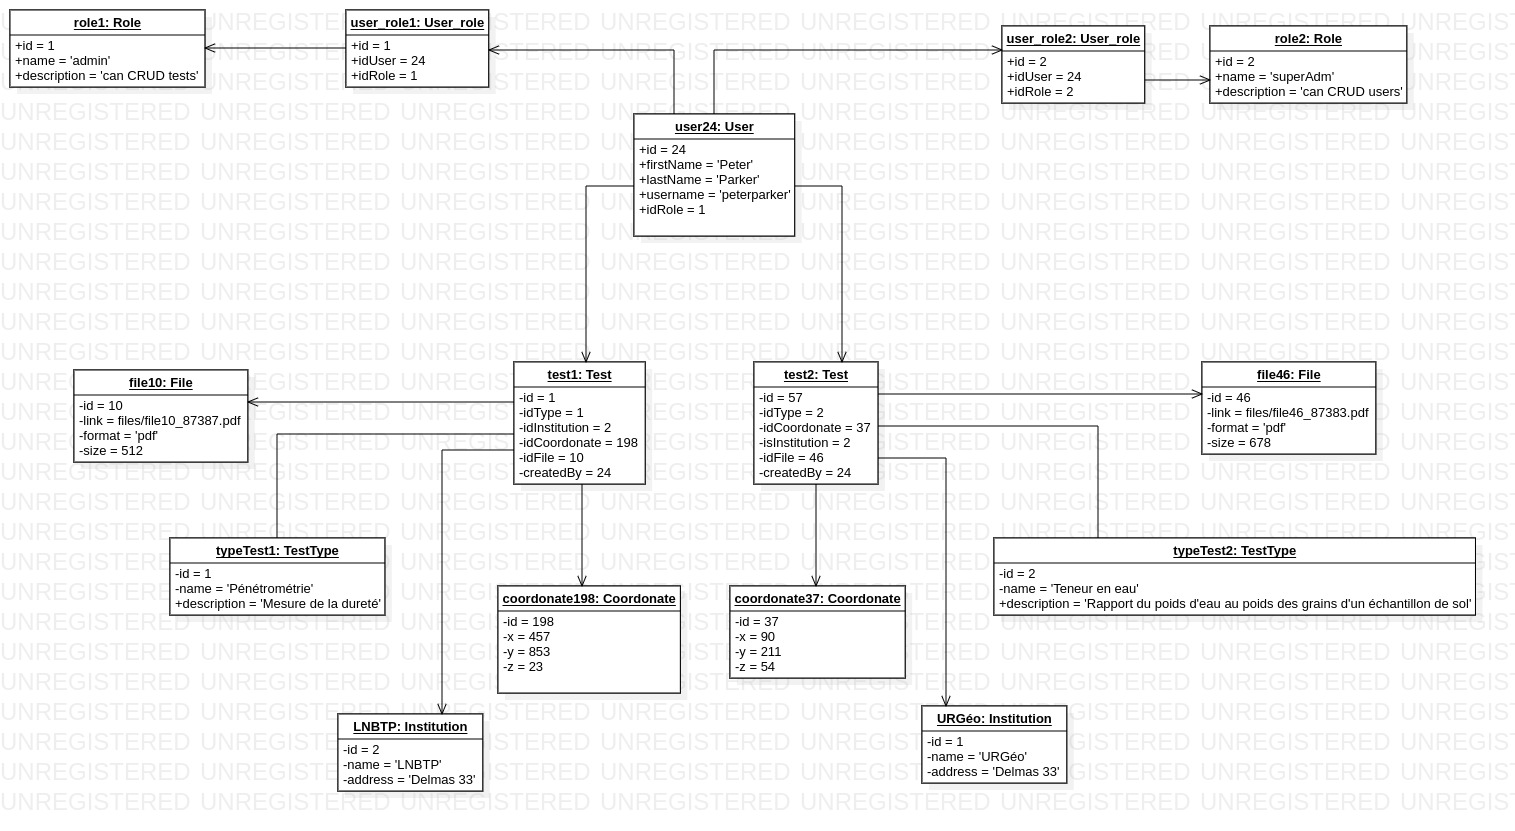
\includegraphics[width=1\textwidth]{images/Analyse_des_besoins/ObjectDiagram.jpg}
        \caption{Cheminement de la solution}
        \label{fig:ObjectDiagram}
    \end{figure}

    \subsection{Diagramme d'activités}
    Le diagramme d'activités a pour rôle principal de représenter graphiquement 
    le comportement du système. Il facilite ainsi la compréhension de chacun en prenant 
    en compte l'interaction des acteurs tant internes qu'externes. 
    \par 
    Dans le cadre d'un projet d'automatisme, nous nous serions probablement tournés vers un 
    diagramme d'états-transitions qui saurait prendre en compte chaque état du système afin d'en prévenir
    la prochaine action. Mais là, l'interaction obligatoire d'un acteur nous oblige à 
    considérer le comportement d'un système basé sur la programmation orientée objet. Il 
    montre les actions à un très haut niveau d’abstraction avec les interactions entre elles \cite{conan2015introduction}. 
    Notre diagramme se présente alors comme suit:
    

    \subsection{Diagramme de séquence}
    Les diagrammes de séquence sont une solution de modélisation 
    dynamique populaire dans UML car ils se concentrent spécifiquement 
    sur les lignes de vie, ou les processus et les objets qui vivent 
    simultanément, et les messages échangés entre eux pour exécuter 
    une fonction avant la fin de la ligne de vie. 
    \par
    Un diagramme de séquence est un type de diagramme d'interaction car 
    il décrit comment et dans quel ordre un groupe d'objets fonctionne 
    ensemble. Ces diagrammes sont utilisés par les développeurs de 
    logiciels et les professionnels pour comprendre les exigences 
    d'un nouveau système ou pour documenter un processus existant. 
    Les diagrammes de séquence sont parfois appelés diagrammes d'événements 
    ou scénarios d'événements.
    \par 
    Le but principal d'un diagramme de séquence est de définir des séquences 
    d'événements qui aboutissent à un résultat souhaité. L'accent est moins mis 
    sur les messages eux-mêmes que sur l'ordre dans lequel les messages se produisent; 
    néanmoins, la plupart des diagrammes de séquence communiqueront quels messages sont 
    envoyés entre les objets d’un système ainsi que l’ordre dans lequel ils se 
    produisent \cite{citeseqdiag}.
    \paragraph{}
    \textit{Les principales informations contenues dans un sont les messages échangés 
    entre les lignes de vie, présentés dans un ordre chronologique. Ainsi, 
    contrairement au diagramme de communication, le temps y est représenté 
    explicitement par une dimension (la dimension verticale) et s'écoule de 
    haut en bas\cite{}.}
    \begin{figure}[t]
        \centering
        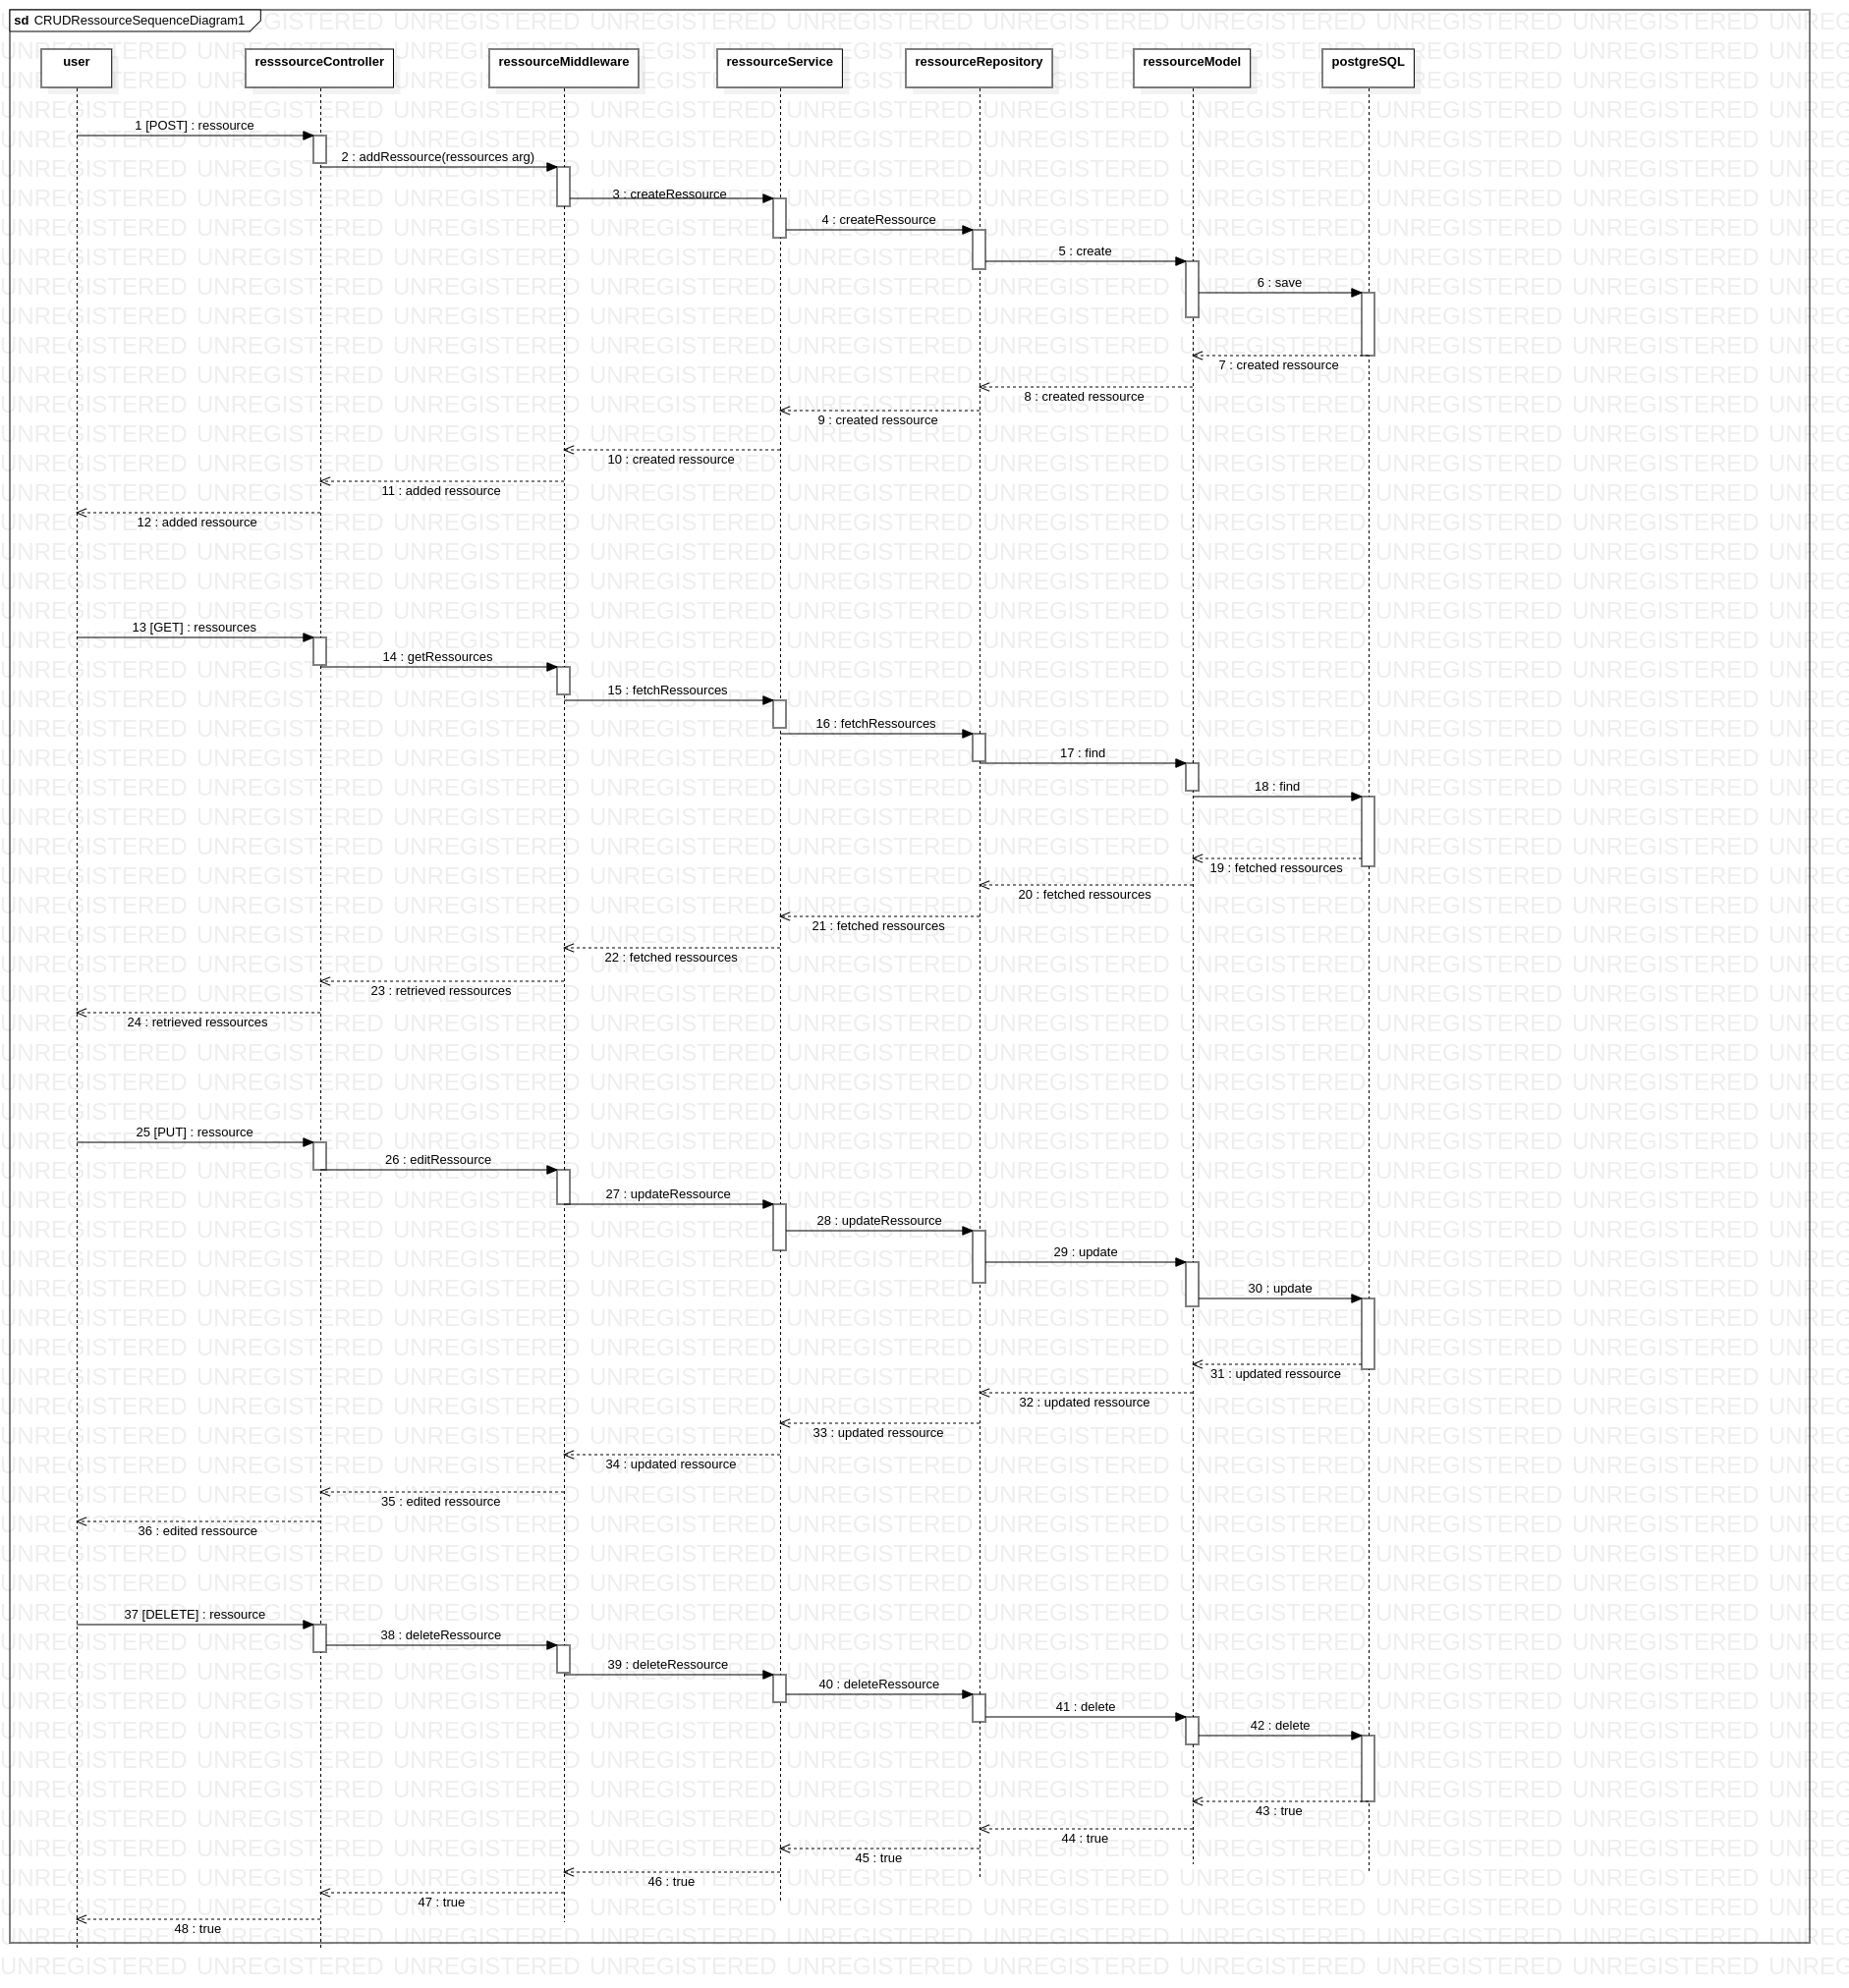
\includegraphics[width=1\textwidth]{images/Analyse_des_besoins/CRUDRessourceSequenceDiagram1.png}
        \caption{Diagramme des séquences : CRUD ressources}
        \label{fig:CRUDRessourceSequenceDiagram1}
    \end{figure}

    \begin{figure}[t]
        \centering
        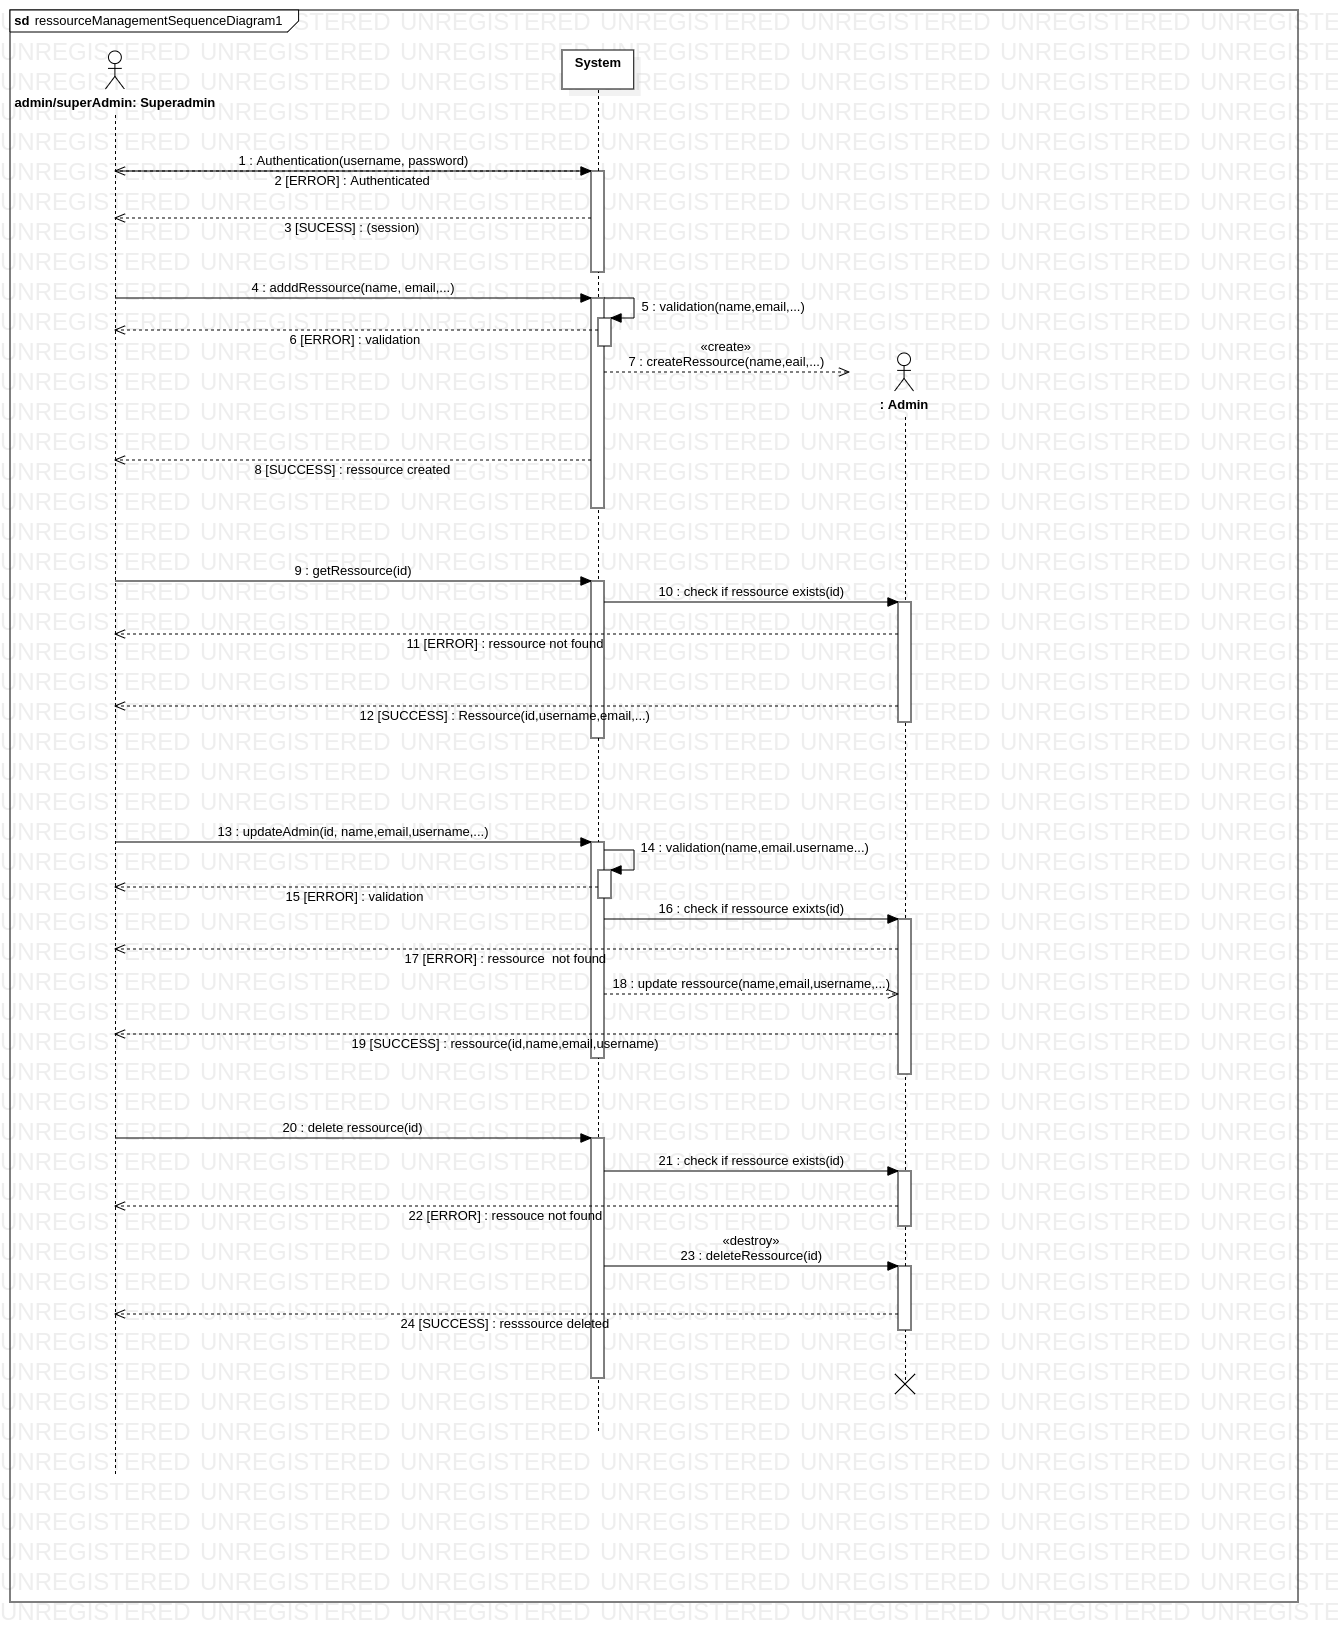
\includegraphics[width=1\textwidth]{images/Analyse_des_besoins/ressourceManagementSequenceDiagram1.png}
        \caption{Diagramme des séquences : gestion des ressources}
        \label{fig:ressourceManagementSequenceDiagram1}
    \end{figure}

    \begin{figure}[t]
        \centering
        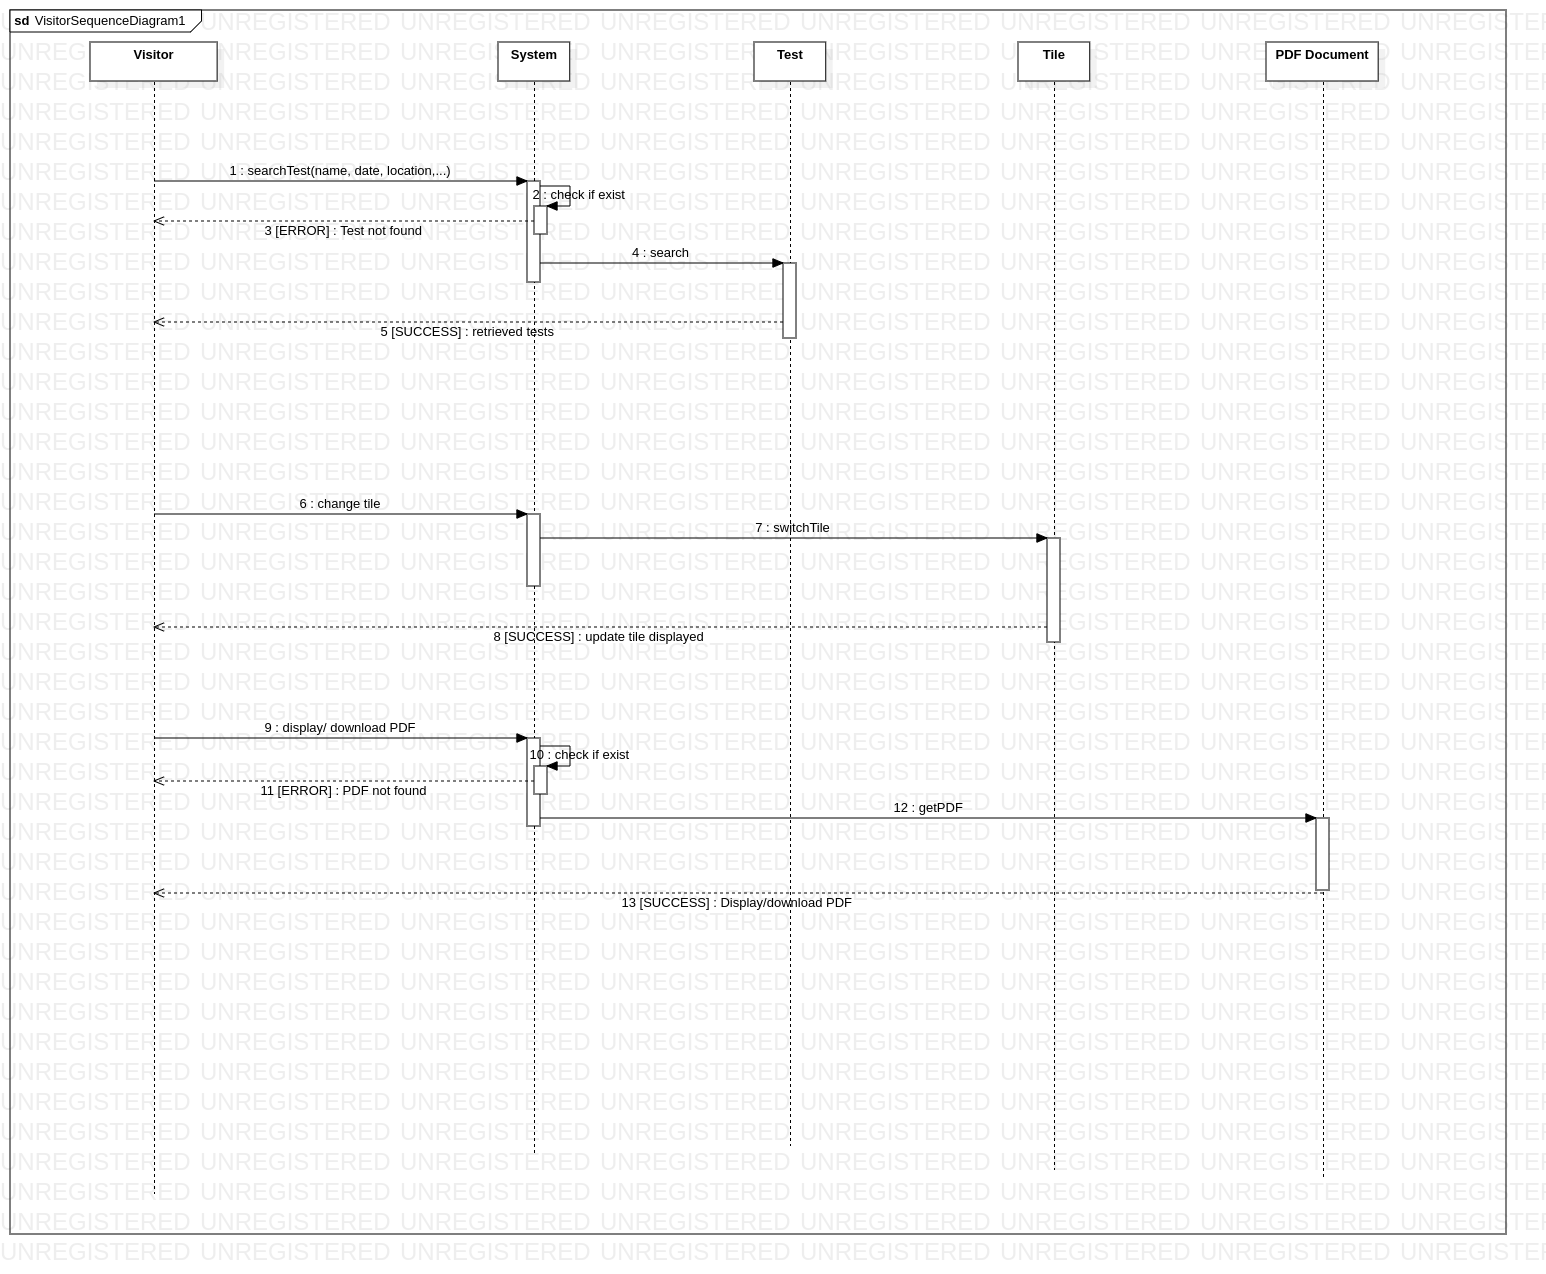
\includegraphics[width=1\textwidth]{images/Analyse_des_besoins/VisitorSequenceDiagram1.png}
        \caption{Diagramme des séquences : visiteur}
        \label{fig:VisitorSequenceDiagram1}
    \end{figure}
        
 

\section{E Documents de validation}
Lorem ipsum dolor sit amet, consectetur adipiscing elit. Mauris at ultrices purus. Donec finibus metus et augue sodales posuere. Proin sit amet turpis dictum, iaculis felis in, scelerisque massa. Nullam aliquam nunc eget fringilla volutpat. Integer et mauris et massa imperdiet scelerisque mollis at sapien. Donec condimentum felis eget sagittis ultricies. Nunc laoreet augue id consectetur vulputate. Cras sagittis aliquam risus sit amet tempus. Curabitur finibus neque eget magna efficitur, sed dignissim quam sagittis. Ut euismod justo id gravida pulvinar. Ut urna magna, auctor maximus volutpat ac, elementum sed mi.
    \section{Objectifs}
    Lorem ipsum dolor sit amet, consectetur adipiscing elit. Mauris at ultrices purus. Donec finibus metus et augue sodales posuere. Proin sit amet turpis dictum, iaculis felis in, scelerisque massa. Nullam aliquam nunc eget fringilla volutpat. Integer et mauris et massa imperdiet scelerisque mollis at sapien. Donec condimentum felis eget sagittis ultricies. Nunc laoreet augue id consectetur vulputate. Cras sagittis aliquam risus sit amet tempus. Curabitur finibus neque eget magna efficitur, sed dignissim quam sagittis. Ut euismod justo id gravida pulvinar. Ut urna magna, auctor maximus volutpat ac, elementum sed mi.
    \section{Protocole}
    Lorem ipsum dolor sit amet, consectetur adipiscing elit. Mauris at ultrices purus. Donec finibus metus et augue sodales posuere. Proin sit amet turpis dictum, iaculis felis in, scelerisque massa. Nullam aliquam nunc eget fringilla volutpat. Integer et mauris et massa imperdiet scelerisque mollis at sapien. Donec condimentum felis eget sagittis ultricies. Nunc laoreet augue id consectetur vulputate. Cras sagittis aliquam risus sit amet tempus. Curabitur finibus neque eget magna efficitur, sed dignissim quam sagittis. Ut euismod justo id gravida pulvinar. Ut urna magna, auctor maximus volutpat ac, elementum sed mi.
    \section{Attentes}
    Lorem ipsum dolor sit amet, consectetur adipiscing elit. Mauris at ultrices purus. Donec finibus metus et augue sodales posuere. Proin sit amet turpis dictum, iaculis felis in, scelerisque massa. Nullam aliquam nunc eget fringilla volutpat. Integer et mauris et massa imperdiet scelerisque mollis at sapien. Donec condimentum felis eget sagittis ultricies. Nunc laoreet augue id consectetur vulputate. Cras sagittis aliquam risus sit amet tempus. Curabitur finibus neque eget magna efficitur, sed dignissim quam sagittis. Ut euismod justo id gravida pulvinar. Ut urna magna, auctor maximus volutpat ac, elementum sed mi.


\section{Diagrammes d'activité}
\lipsum[1]

\begin{figure}[t]
    \centering
    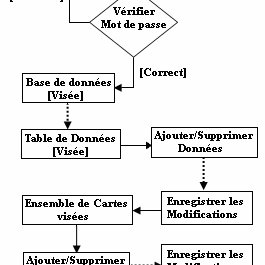
\includegraphics[width=1\textwidth]{diagrammeActivite}
    \label{image-diagrammeActivite}
    \caption{Diagramme d'activites}
    \end{figure}


\chapter{Implémentation}
        \section{Choix des technologies}
        Au cours de la réalisation d'un logiciel numérique,
        l'une des étapes les plus importantes est de choisir la bonne pile technologique. 
        Pourquoi? Parce qu'il s'agit de créer un produit qui ne consiste pas uniquement
        à concevoir une interface utilisateur agréable et une expérience utilisateur 
        pratique; il s'agit également de concevoir un produit stable, sécurisé et 
        maintenable qui, non seulement est en mesure de charmer les utilisateurs mais encore, vous 
        permettra de faire évoluer l'entreprise.
        \paragraph{}
        Chaque couche de l'application est construite au-dessus d'une autre, 
        formant une pile. Cela rend les technologies Web fortement dépendantes 
        les unes des autres. L'image \ref{fig:pile} montre les principaux éléments constitutifs 
        d'une pile technologique typique; cependant, il peut y avoir d'autres éléments de 
        soutien impliqués.
        \begin{figure}[t]
                \centering
                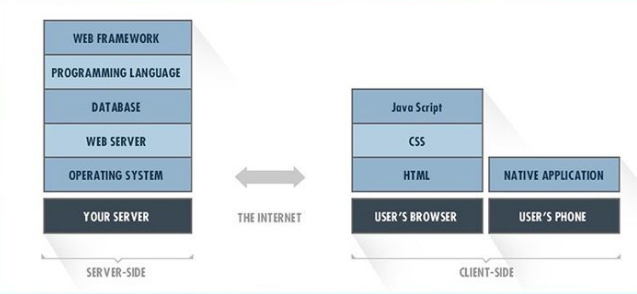
\includegraphics[scale=0.5]{images/Implementation/pile.png}
                \caption{Modèle du cycle de vie en cascade \cite{Bulatovych}}
                \label{fig:pile}
        \end{figure}
        \subsection{Frontend}
        L'interface utilisateur est également appelée côté client, car les utilisateurs voient et interagissent 
        avec cette partie d'une application. Pour une application web, cette interaction s'effectue 
        dans un navigateur web et est possible grâce à de nombreux outils de programmation (Tableau \ref{tab:techoFrontend}). 
        Les applications Web destinées aux clients sont généralement créées à l'aide d'une combinaison 
        de JavaScript, HTML et CSS.
        \paragraph{Outils que nous utilisons pour le développement frontend:}
        \paragraph{HTML: }
        (Hypertext Markup Language) est un langage de programmation utilisé pour décrire 
        la structure des informations présentées sur une page Web. 
        \textit{Le World Wide Web est aujourd'hui l'une des sources d'information les plus 
        importantes. La plupart des données sur le Web sont disponibles sous forme de 
        pages encodées dans des langages de balisage tels que HTML destinés aux 
        navigateurs visuels \cite{yang2003html}.} 
        \par 
        Pour la réalisation de GeoTechMap, nou utilisons HTML5 qui est la cinquième et dernière 
        édition recommandée par le World Wide Web Consortium (W3C) \cite{brooks2010world}.
        \paragraph{CSS: }
         (Cascading Style Sheets) est un langage de feuille de style qui décrit 
        l'apparence et la mise en forme d'un document écrit en HTML. CSS est utilisé 
        pour annoter du texte et incorporer des balises dans des documents électroniques stylisés.
        Le CSS est encore plus important car il doit être pris en compte pour rendre l'applicatgion responsive.
        L'interface utilisateur doit pouvoir s'adapter à n'importe quelle dimention d'écran 
        d'autant plus que nous constatons la montée du trafic web via les téléphones mobiles (Figure \ref{fig:statMobile}).
        \begin{figure}[t]
                \centering
                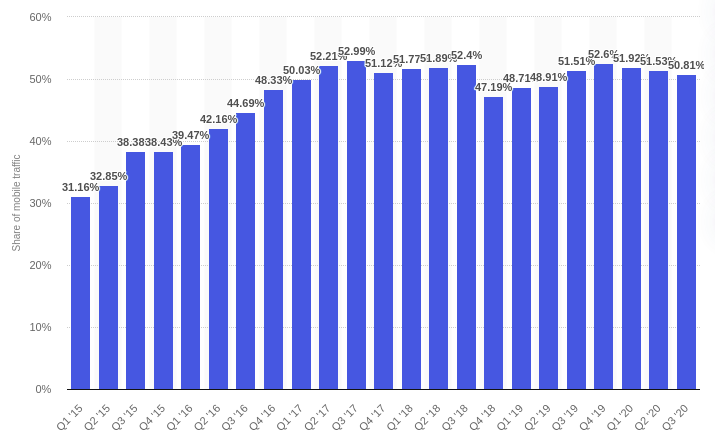
\includegraphics[scale=0.5]{images/Implementation/statMobile.png}
                \caption{
                        Pourcentage du trafic du site Web sur les appareils 
                        mobiles dans le monde du 1er trimestre 2015 au 3ème trimestre 2020 \cite{linkstatmobile}}
                \label{fig:statMobile}
        \end{figure}
        \paragraph{JavaScript (ou JS): }
         C'est la troisième technologie principale pour créer 
        l'interface d'une application Web. JavaScript est couramment utilisé pour créer des 
        pages Web dynamiques et interactives. En d'autres termes, il permet des animations 
        Web simples et complexes, qui contribuent grandement à une expérience utilisateur 
        positive.
        \par
        \textit{JavaScript est devenu le langage de facto pour la programmation Web côté client \cite{gardner2012towards}.}
        \paragraph{React: }
        C'est une bibliothèque JavaScript pour créer des interfaces utilisateur.
        ReactJS offre des solutions élégantes à certains des problèmes les plus 
        persistants de la programmation frontend, vous permettant de créer facilement 
        des applications Web dynamiques et interactives. Il est rapide, évolutif, flexible, 
        puissant et dispose d’une solide communauté de développeurs qui se développe 
        rapidement. \textit{Il s'agit actuellement de la bibliothèque JS frontale la plus populaire \cite{aggarwal2018modern}.}  
        \par    
        \begin{table}
                \centering
                \begin{tabular}{|p{0.30\linewidth}|p{0.10\linewidth}|p{0.60\linewidth}|}
                \hline
                        \textbf{Technologie}&\textbf{Version}&\textbf{Détails}\\
                        \hline
                        HTML&
                        5&
                        HTML5 est conçu pour rendre le développement de ces applications Web 
                        riches plus facile, plus naturel et plus logique, où les développeurs 
                        peuvent concevoir et créer une seule fois, et les déployer n'importe où. 
                        HTML5 rend également les applications Web plus utilisables, car il supprime 
                        le besoin de plugins \cite{wang2013definitive}.
                        \\
                        \hline
                        CSS&
                        3&
                        bla
                        \\
                        \hline
                        JS&
                        ES6&
                        « ES » est l’abréviation d’ECMAScript, le standard sur lequel repose JavaScript.
                        Tous les navigateurs modernes supportent l’ES6 depuis un moment, et les 
                        frameworks majeurs (Angular, React, Vue…) utilisent tous cette nouvelle version de JavaScript
                        \\
                        \hline
                        React&
                        17&
                        \textit{Bien que React v17 ne propose aucune nouvelle fonctionnalité, 
                        il établit une base solide pour les versions à venir en abordant directement 
                        l'expérience de mise à niveau et en alignant plus étroitement le comportement 
                        de React sur les navigateurs modernes \cite{Vardhan2020}.}
                        \\
                        \hline
                      
                \end{tabular}
                \caption{Les technologies utilisées pour le développement du frontend de GeoTechMap} 
                \label{tab:techoFrontend}
        \end{table}
        \par
        \subsection{Backend}
        Le backend, qui n'est pas visible pour les utilisateurs finaux, implique la logique métier, 
        l'authentification, la gestion de la base de données et les synchronisations avec 
        l'application cliente. Également appelé côté serveur, il est composé d'un serveur, d'une base 
        de données et d'applications qui s'exécutent dessus.
        \par 
        Même si le backend fonctionne en dehors de la scène et n'est pas visible pour les utilisateurs, 
        c'est le moteur qui pilote votre application et met en œuvre sa logique. Le serveur Web, qui 
        fait partie du backend, accepte les requêtes d'un navigateur, traite ces requêtes selon une 
        certaine logique, se tourne vers la base de données si nécessaire et renvoie le contenu pertinent. 
        \par 
        \textit{Les applications Web sophistiquées d'aujourd'hui ne peuvent pas fonctionner sans
         les services frontaux et backend \cite{abdullah2014frontend}.}

        \subsubsection{Système d'exploitation}
        Le système d'exploitation installé sur le serveur est le plus souvent Windows ou Linux.
        Dans notre cas, il s'agit de Linux pour plusieurs raisons.
        \textit{Les systèmes Linux ont tendance à être plus dynamiques que les 
        systèmes Windows, en raison du taux rapide de mises à jour  
        dans de nombreux projets Linux \cite{ovadia2014linux}.}
        \par
        En effet, la liste des avantages de Linux 
        est longue. Citons entre autre \cite{advlinux} :
        \begin{itemize}
                \item \textbf{Open source: }
                Comme il est open source, son code source est facilement disponible. 
                Toute personne ayant des connaissances en programmation peut personnaliser 
                le système d'exploitation. On peut contribuer, modifier, distribuer et 
                améliorer le code dans n'importe quel but.
                \item \textbf{Sécurité: }
                La fonction de sécurité Linux est la principale raison pour laquelle c'est 
                l'option la plus favorable pour les développeurs. Ce n'est pas complètement 
                sûr, mais il est moins vulnérable que d'autres. Chaque application doit 
                être autorisée par l'utilisateur administrateur. Le virus n'est pas exécuté 
                tant que l'administrateur n'a pas fourni le mot de passe d'accès. Les systèmes 
                Linux ne nécessitent aucun programme antivirus.
                De plus, linux est aussi mieux protégé contre les virus car il a un grand 
                nombre de développeurs open source qui gardent un œil sur les choses liées aux 
                virus. Si un code source doit être mis à jour, cela se fait en un rien de temps.
                \item \textbf{Léger: }
                Linux est léger. Les exigences pour exécuter Linux sont bien inférieures à 
                celles des autres systèmes d'exploitation. Sous Linux, l'empreinte mémoire et 
                l'espace disque sont également inférieurs. En règle générale, 
                la plupart des distributions Linux ne nécessitaient que 128 Mo de RAM, 
                soit environ la même quantité d'espace disque.
                \item \textbf{Stabilité: }
                Linux est plus stable que les autres systèmes d'exploitation. Linux n'a pas 
                besoin de redémarrer le système pour maintenir les niveaux de performances. 
                Il raccroche ou ralentit rarement.
                \item \textbf{Convient aux programmeurs: }
                Il prend en charge presque tous les langages de programmation les plus utilisés 
                tels que C / C ++, Java, Python, Ruby, etc. De plus, il offre une vaste gamme 
                d'applications utiles pour le développement.
                Les programmeurs préfèrent le terminal Linux à la ligne de commande Windows. 
                Le gestionnaire de paquets sur le système Linux aide les programmeurs à 
                comprendre comment les choses sont faites. Le script bash est également une 
                fonctionnalité pour les programmeurs. Il prend également en charge SSH, 
                ce qui permet de gérer rapidement les serveurs.
                
        \end{itemize}
        La liste est longue (grande communauté, réseau, compatibilité, installation, etc). Par conséquent
        notre choix s'est porté sur le système d'explotation le mieux adapté à ce projet, en l'occurence linux.

        \subsubsection{Server web}
        Un composant qui synchronise la communication entre les navigateurs, les applications mobiles et 
        le serveur principal. Il utilise HTTP / HTTPS pour transférer des données entre les deux extrémités.
        Dans notre cas,  nos servers sont des instances chez AWS  nommées EC2. 

        Une instance EC2 est un serveur virtuel dans Elastic Compute Cloud (EC2) d'Amazon pour exécuter 
        des applications sur l'infrastructure Amazon Web Services (AWS).
        \par 
Le cloud offre de nombreux avantages techniques et économiques par rapport à  
       d'autres plateformes qui commencent tout juste à être identifiées. Ils combinent la 
        personnalisation des machines virtuelles, l'évolutivité et le partage des ressources,
         ainsi que la stabilité et l'économie du logiciel en tant que service 
         (Platfom as a Service: SaaS) \cite{juve2009scientific}.

         \subsubsection{Base de données}
         Une base de données est une collection organisée d'informations. Les bases de données
         comprennent généralement des agrégations d'enregistrements de données ou de fichiers. 
         \par 
         Il existe différents types de bases de données utilisées pour stocker différentes 
         variétés de données: centralisée, distribuée, relationnelle, NoSQL, 
         orientée object, ... \cite{typedb}
         \par 
         Pour la réalisation de GeoTechMap, nous faisons le choix d'une base de données relationnelle.
         En effet, cette base de données est basée sur le modèle de données relationnel, qui stocke les 
         données sous forme de lignes (tuple) et de colonnes (attributs), et forme ensemble une table 
         (relation). Une base de données relationnelle utilise SQL pour stocker, manipuler et conserver 
         les données. Chaque table de la base de données 
         contient une clé qui rend les données uniques des autres. MySQL, Microsoft SQL Server, Oracle, ... 
         sont des exemples de bases de données relationnelles.
         \par 
         \textit{La technologie des bases de données relationnelles offre des améliorations considérables 
         de la productivité tant pour les utilisateurs finaux que pour les programmeurs d'applications \cite{codd1989relational}.}
         \paragraph{Propriétés d'une base de données relationnelle}
         Il existe quatre propriétés communément connues d'un modèle relationnel appelées propriétés ACID \cite{typedb}, où:
         \begin{itemize}
                 \item \textbf{A signifie Atomicité: }
                  Cela garantit que l'opération de données se terminera 
                 avec succès ou échec. Il suit la stratégie du «tout ou rien». Par exemple, 
                 une transaction sera soit validée, soit abandonnée.
                 \item \textbf{C signifie Cohérence: }
                  Si nous effectuons une opération sur une donnée, 
                 sa valeur avant et après l'opération doit être préservée. Par exemple, 
                 le solde du compte avant et après la transaction doit être correct.
                 \item \textbf{I signifie Isolation: }
                 Il peut y avoir des utilisateurs  
                 qui accèdent simultanément aux données dans de la base de données. 
                 Ainsi, l'isolement entre les données doit rester effectué. Par exemple, 
                 lorsque plusieurs transactions se produisent en même temps, les effets 
                 d'une transaction ne doivent pas être visibles pour les autres 
                 transactions de la base de données.
                 \item \textbf{D signifie Durabilité: }
                 Il garantit qu'une fois l'opération terminée et validé les données, 
                 les modifications de données doivent rester permanentes.

         \end{itemize}
         \paragraph{Pourquoi PostgreSQL comme SGBD ?}
         \paragraph{}
         Selon le site officiel de PostgreSQL \cite{psql},
         PostgreSQL est un puissant système de base de données relationnelle objet et open 
         source qui utilise et étend le langage SQL combiné à de nombreuses fonctionnalités
          qui stockent et mettent à l'échelle en toute sécurité les charges de travail de 
          données les plus complexes.
          \par 
          PostgreSQL est livré avec de nombreuses fonctionnalités destinées à aider les 
          développeurs à créer des applications, les administrateurs à protéger 
          l'intégrité des données et à créer des environnements tolérants aux pannes, 
          et vous aider à gérer vos données, quelle que soit la taille de l'ensemble de 
          données. En plus d'être gratuit et open source, PostgreSQL est hautement extensible.
          \par 
          PostgreSQL est populaire auprès des développeurs en raison de nombreuses fonctionnalités
           telles que: le partitionnement natif, les requêtes parallèles, la prise en charge 
           de wrappers de données étrangers, de puissantes fonctionnalités JSON, le streaming et 
           la réplication logique et la disponibilité de nombreux outils open source,
            les sauvegardes et la surveillance.
            \paragraph{}
            De plus, plusieurs bases de données géotechnique ont été 
            déjà réalisées avec PostgreSQL et ce fut un succès. Tel est le cas du
            "développement de la base de données getechnical du sous-sol de Bangkok 
            en utilisant GRASS-GIS" \cite{panoot2001development}.
        \subsubsection{Application backend}
        \paragraph{Langage de programmation: }
        Différents langages de programmation peuvent être utilisés pour développer l'application 
        backend. Les plus populaires sont Java, Python, JavaScript, PHP.
        \paragraph{Pourquoi choisur JAva ?: }
        \begin{itemize}
                \item \textbf{Orienté objet: } En Java, tout est un objet. Java est extensible 
                car il basé sur le modèle des objects.
                \item \textbf{ Indépendant de la plateforme: } Contrairement à de nombreux 
                autres langages de programmation (C, C ++), lorsque Java est compilé, il ne se 
                compile pas sur un ordinateur spécifique à une plate-forme, mais est en 
                bytecode indépendant du système. Ce bytecode est distribué sur le Web 
                et est interprété par la machine virtuelle (JVM) sur n'importe quelle 
                plate-forme qui l'exécute. un programme Java peut être exécuté dans n'importe quel 
                environnement grâce au JVM.
                \par 
                La signification de indépendant de la plateforme est que le code compilé par java (byte code) 
                peut s'exécuter sur tous les systèmes d'exploitation.
                Un programme est écrit dans une langage qui est compréhensible par l'homme. 
                Il peut contenir des mots, des phrases, etc. que la machine ne comprend pas. 
                Pour que le code source soit compris par la machine, il doit être dans un langage 
                compris par les machines, généralement un 'langage machine'. Alors, voici le rôle 
                d'un compilateur. Le compilateur convertit le langage de haut niveau (langage humain) 
                en un format compris par les machines. Par conséquent, un compilateur est un programme 
                qui traduit le code source d'un autre programme d'un langage de programmation en code exécutable.
                Ce code exécutable peut être une séquence d'instructions machine qui peuvent être exécutées 
                directement par le CPU, ou il peut être une représentation intermédiaire qui est interprétée 
                par une machine virtuelle. Cette représentation intermédiaire en Java est le Java Byte Code \cite{java}.
                \item \textbf{Sécurité: } La sécurité en Java commence au niveau des fonctionnalités 
                du langage. Cela nous permet d'écrire du code sécurisé et de bénéficier de nombreuses fonctionnalités 
                de sécurité implicites:
                        \begin{itemize}
                                \item \textbf{Type de donnée static: } Java est un langage à typage statique, ce qui réduit les 
                                possibilités de détection d'erreurs liées au type lors de l'excution.
                                \item \textbf{ Modificateurs d'accès: } Java nous permet d'utiliser 
                                différents modificateurs d'accès tels que public et privé pour contrôler l'accès aux champs, 
                                méthodes et classes.
                                \item \textbf{Gestion automatique de la mémoire: } Java a une gestion de 
                                la mémoire basée sur le garbage collection, donc les développeurs n'ont plus à s'occuper de la
                                 gestion manuelle.
                                 \item \textbf{Gestion automatique de la mémoire: } Java a une gestion de 
                                la mémoire basée sur le garbage collection, donc les développeurs n'ont plus à s'occuper de la
                                 gestion manuelle.
                                 \item ... \cite{java}
                        \end{itemize}
                \item \textbf{Robuste: }  Java s'efforce d'éliminer les situations sujettes aux erreurs en mettant principalement l'accent 
                sur la vérification des erreurs au moment de la compilation et les tests d'exécution.
                \item \textbf{Multithread: }: Avec la fonction multithread de Java, vous pouvez écrire des programmes capables d'exécuter plusieurs 
                tâches simultanément. Cette fonctionnalité permet aux développeurs de créer des applications interactives qui peuvent 
                fonctionner sans problème.
                \item \textbf{Documentation: }: Javadoc est une excellente documentation qui offre aux développeurs des informations étendues sur les extensions Java.
                Javadoc a été spécialement développé pour faciliter le codage pour les développeurs et utiliser facilement un ensemble de classes.
                
        \end{itemize}
        \paragraph{}
        \textit{La valeur de Java peut être calculée à partir du fait que des entités populaires 
        telles que Facebook, LinkedIn, eBay et Amazon font toutes confiance à Java pour leurs 
        sites Web. Et la popularité de ces plateformes n'est pas nouvelle pour nous.
        Ce qui rend Java plus populaire, c'est que le langage de codage est suffisamment 
        compatible pour être utilisé pour les applications d'entreprise en prenant en charge 
        des technologies telles que l'IoT, l'IA, machine learning, etc. \cite{whyjava}.}
        
        \subsubsection{Framework }
        Un framework Java est un logiciel qui fournit un moyen extensible et standardisé de créer 
        et de déployer des applications. Selon le framework, ils peuvent inclure des outils, 
        des compilateurs, des bibliothèques et des API. Pour le développement Web Java, les développeurs utilisent u
        ne variété de frameworks (Spring, Hibernate, Struts, Wicket, GWT, etc) pour répondre aux besoins de 
        leur application.
        \paragraph{Spring boot}
        \paragraph{}
        Spring Boot est un framework open source basé sur Java. Spring Boot fournit une bonne plate-forme aux développeurs Java pour 
        développer une application Spring autonome et de qualité production que vous pouvez simplement exécuter. 
        \paragraph{Pourquoi Spring Boot ?}
        \paragraph{}
        Nous avons choisi Spring Boot en raison des fonctionnalités et des avantages qu'il offre, parmis lesquels :
        \begin{itemize}
                \item Il offre un moyen flexible de configurer les Java Beans\footnote{
                        Une propriété JavaBean est une fonction nommée accessible par l'utilisateur de l'objet. 
                        La fonction peut être de n'importe quel type de données Java, contenant les classes que 
                        vous définissez. Par exemple, si le nom de la propriété est firstName, le nom de la méthode 
                        serait getFirstName () pour lire cette propriété.
                }, les
                 fichier XML et les transactions de base de données.
                \item Il fournit un puissante gestion des processus batch et des points d'accès REST.
                \item Dans Spring Boot, tout est configuré automatiquement; aucune configuration manuelle n'est nécessaire.
                \item Il offre une application basée sur les annotations \footnote{
                        Java Annotation is a tag that represents the metadata i.e. attached with class, interface, methods or fields to indicate 
                        some additional information which can be used by java compiler and JVM \cite{annotation}.
                }.
                \item Facilite la gestion des dépendances.
                \item Il comprend un Embedded Servlet Container(conteneur de servlet intégré).
        \end{itemize}
        \subsubsection{Gestion des utilisateurs}
        L'authentification et la sécurité des services sont des fonctionalés incontournables pour un système comme GeoTechMap.
        Pour gerer tout cela, nous utilisons Keycloak.
        \par 
        \textit{
                Keycloak est une solution open source de gestion des identités et des accès destinée aux applications 
                et services modernes \cite{keycloak}.} 
        \paragraph{}
        Le type d'application que nous développons influence la technologie que nous selectionons.
        Plusieurs facteurs ont joué dans le choix des technologies choisies. L'objectif des combinaisons
        réalisées n'est que l'optimisation de l'implementation du système GeoTechMap.
        \section{La hiérarchie dans l'application}
        \lipsum[1]
        \section{Ergonomie}
        % Interface utilisateur
        \lipsum[1]
        \section{Déploiement}
        \lipsum[1]
        \section{Sécurité du système}
        % -securitaire
        % -high reliability
        % -high scalability
        \lipsum[1]
        \section{Limitations du système}
        \lipsum[1]
        \section{Coûts}
        \lipsum[1]
    



\chapter{Conclusion}
        \section{Ameliorations futures}
        \subsection{Suite du projet}
        \lipsum[1]
         \subsection{Défis rencontrés}
        \lipsum[1]
         \subsection{Propositions}
        \lipsum[1]
        \section{Conclusion}
        \lipsum[1]


\bibliographystyle{plain}
\bibliography{bibliographie}

\end{document}